\documentclass[11pt,a4paper]{article}
\usepackage[margin=1in]{geometry}
\usepackage{amsmath,amssymb}
\usepackage{booktabs}
\usepackage{array}
\usepackage{listings}
\usepackage{xcolor}
\usepackage[colorlinks=true,linkcolor=black,urlcolor=blue]{hyperref}
\usepackage{parskip}
\usepackage{tikz}
\usetikzlibrary{positioning,arrows.meta,fit,backgrounds,calc}

\definecolor{ink}{HTML}{1A1A1A}
\definecolor{grey}{HTML}{5F5B54}
\definecolor{pale}{HTML}{F5F3EE}
\definecolor{tensor}{HTML}{1F6F4A}
\definecolor{seq}{HTML}{1F4E8C}
\definecolor{prod}{HTML}{9C3B1B}
\definecolor{hdrbg}{HTML}{D6E4F5}   % headers
\definecolor{bdybg}{HTML}{D5EDDC}   % bodies
\definecolor{linebg}{HTML}{F7D8E3}   % protocol / request line / status line
\definecolor{pathbg}{HTML}{F6E7C1}   % paths

\tikzset{
  srv/.style={draw=ink, fill=white, rounded corners=2pt, inner sep=3.4pt,
              font=\scriptsize\ttfamily, minimum height=5.6mm},
  plan/.style={srv, fill=pale, font=\scriptsize\ttfamily\bfseries},
  op/.style={circle, draw, inner sep=0.6pt, minimum size=6.4mm, font=\footnotesize\bfseries},
  ar/.style={-{Stealth[length=1.8mm]}, semithick, color=grey},
  lbl/.style={font=\tiny\itshape, color=grey},
  capt/.style={font=\scriptsize\bfseries},
  subt/.style={font=\tiny\itshape, color=grey},
}

\definecolor{kw}{RGB}{20,80,160}
\definecolor{cmt}{RGB}{110,110,110}
\definecolor{str}{RGB}{160,60,20}
\definecolor{codebg}{RGB}{246,246,244}

\lstdefinestyle{code}{
  basicstyle=\ttfamily\small,
  keywordstyle=\color{kw}\bfseries,
  commentstyle=\color{cmt}\itshape,
  stringstyle=\color{str},
  breaklines=true,
  frame=leftline,
  framesep=7pt,
  xleftmargin=12pt,
  rulecolor=\color{gray!45},
  backgroundcolor=\color{codebg},
  columns=fullflexible,
  showstringspaces=false,
  keepspaces=true,
  literate=
    {↓}{{$\downarrow$}}1 {↑}{{$\uparrow$}}1
    {→}{{$\rightarrow$}}1 {⊠}{{$\boxtimes$}}1
    {◁}{{$\lhd$}}1 {×}{{$\times$}}1 {—}{{\textemdash}}1 {’}{{'}}1,
}
\lstset{style=code}

% Enforcement badges: compile time / run time / developer discipline.
\definecolor{enfc}{HTML}{1F4E8C}
\definecolor{enfr}{HTML}{1F6F4A}
\definecolor{enfd}{HTML}{9C3B1B}
\newcommand{\badge}[2]{\raisebox{0.05ex}{\fcolorbox{#1}{white}{\textcolor{#1}{\scriptsize\bfseries\,#2\,}}}}
\newcommand{\enfC}{\badge{enfc}{C}}
\newcommand{\enfR}{\badge{enfr}{R}}
\newcommand{\enfD}{\badge{enfd}{D}}

% Keep every code block whole: wrapping each listing in an unbreakable minipage
% makes LaTeX move it to the next page rather than split it across one.
\usepackage{etoolbox}
\BeforeBeginEnvironment{lstlisting}{\par\vspace{0.4\baselineskip}\noindent\begin{minipage}{\linewidth}}
\AfterEndEnvironment{lstlisting}{\end{minipage}\par\vspace{0.4\baselineskip}}

% Terminal trace: literate arrows are mis-placed under columns=fullflexible,
% and a literate glyph opening line 1 is flushed onto its own line -- hence
% keepspaces and the leading space on every line of the block below.
\lstdefinestyle{trace}{
  basicstyle=\ttfamily\small,
  keepspaces=true,
  frame=leftline, framesep=7pt, xleftmargin=12pt,
  rulecolor=\color{gray!45},
  backgroundcolor=\color{codebg},
  literate={↓}{{$\downarrow$}}1 {↑}{{$\uparrow$}}1 {…}{{\ldots}}1,
}

\lstdefinelanguage{TS}{
  morekeywords={type,function,switch,case,return,const,extends,never,interface,let,await,async,export,import,null,unknown,new,try,catch,throw,in,of},
  morecomment=[l]{//},
  morestring=[b]",
}
\lstdefinelanguage{SH}{
  morekeywords={curl,deno,run,export,for,do,done,if,then,fi,echo,sort,head,chmod,cat},
  morecomment=[l]{\#},
  morestring=[b]',
}

\title{\vspace{-2em}Stalin: The Game}
\author{Robin Langer}
\date{1 September 2026}

\begin{document}
\maketitle

\begin{center}
\begin{minipage}{0.88\linewidth}\small\itshape
\textbf{Disclaimer.} I am not an expert at Unix, or at web app development, or at container
combinators, so these notes are just as much for myself as for anybody else.
\end{minipage}
\end{center}
\vspace{1mm}

\section*{Introduction}

Neil Ghani's \emph{Containers for Typed Agentic AI} describes an algebra of interfaces. An
interface is a pair. The first half is the prompts you may send. The second half gives, for each
prompt, the type of reply that would answer it. Such interfaces compose, in four different ways,
all of which appear in this game.

Container theory arose out of dependent type theory, and ``playing around'' with containers is
usually done in a language such as Idris or Lean. This is not what we do in these notes. Instead we
``fake'' dependent types using Unix CLI tools and TypeScript \texttt{async} event handlers.

The division of labour between those two is exact, and to say why we need one definition from the
theory. A \emph{morphism} of containers $(P,R) \to (Q,T)$ is a pair of functions
\[
  u : P \to Q
  \qquad\qquad
  f : (p : P) \to T\,(u\,p) \to R\,p .
\]
The mapping $u$ \emph{delegates} a task. The mapping $f$ \emph{amalgamates} a response. So a
container morphism has two flows, prompts moving forwards and responses moving backwards. Control
flows \emph{down} through $u$. Data flows \emph{back up} through $f$.

And each of our two ordinary things supplies exactly one of those flows.

\textbf{CLI tools:} The forward map $u$ on shapes is implemented as a Unix CLI tool call.

This works because a command-line tool is already a container. It receives one prompt, its
argument vector. It produces a response whose \emph{type depends on which prompt it was}.

For example. The command \texttt{git log} answers with a list of commits. The command
\texttt{git status} answers with a working tree. Those are not the same kind of thing, and which
kind you get is fixed by the word after \texttt{git}. That is $(p : P) \to R\,p$, with $P$ the
subcommands and $R$ the result type of each. The interface $(P, R)$ is what \texttt{--help}
prints.

\textbf{TypeScript \texttt{async} event handlers:} The backwards map $f$ on positions is
implemented with TypeScript \texttt{async} event handlers. Each TypeScript \texttt{async} event
handler ``hangs'' on the result of the next TypeScript \texttt{async} event handler in the chain.
When a ``leaf'' at the end of the chain finally evaluates to an actual response, this response
``propagates backwards'' up the chain of TypeScript \texttt{async} event handlers.

\section{The Unix philosophy, pipes, and CLI tools}
\label{sec:unix}

In case the reader is a little rusty, we begin with a brief review of the Unix this note leans
on. What a process is. How one reaches the world outside itself. How two of them are joined
together. Why a command-line tool has the shape it has. None of this is specific to the game
\texttt{stalin}. All of it is used by the game. The game comes later, once the concepts are in
place.

Each part below introduces one idea and, where it helps, one small example that illustrates
only that idea. Nothing is used before it has been introduced.

\subsection*{A process}

A \emph{process} is one running program, together with everything the kernel keeps on its
behalf. Its memory. Its position in the code. Its identity, meaning which user it runs as. And a
number.

A program is a file sitting on a disk, and does nothing. A process is that file in motion. Run the
same program twice and you have two processes. They share nothing and cannot see each other.

The number is the process's \emph{pid}. It is how anything outside the process refers to it, and
there is no other handle. To stop a program you send a signal to its pid.

\subsection*{User space and kernel space}

A running machine is divided in two. Your code executes in \emph{user space}, where it may
compute freely and touch nothing. It cannot address a disk, a network card, or another process's
memory. The processor is in a mode that forbids it. The \emph{kernel} executes in kernel space,
where it may touch everything. The division is enforced by the hardware, not by convention.

There is exactly one interface between the two. It is the \emph{system call}. It suspends your
process, switches the processor into kernel mode, runs kernel code on your process's behalf, and
returns. Every effect a program has on the world outside its own memory is a system call. There is
no other mechanism.

\subsection*{\texttt{read} and \texttt{write}}

That interface could have been wide. It is in fact very narrow. The two calls that matter most
are these:

\begin{lstlisting}[language=SH]
read (n, buffer, count)   -- give me up to count bytes from the thing numbered n
write(n, buffer, count)   -- take these count bytes and put them in the thing numbered n
\end{lstlisting}

Each takes a number identifying something already open, a place to put bytes or take them from,
and how many. Between them they are very nearly the whole interface to the outside world. What that
number is, and where it comes from, is the subject of two subsections below.

\subsection*{Everything is a file}

Why should two calls be enough? Because of a design decision usually stated as a slogan.
\textbf{Everything is a file.} A file on a disk, a terminal, a network connection, a source of
random bytes. All of them are presented to user space through the same interface. So the same two
calls reach all of them.

The slogan overstates itself in one respect, and it is worth being precise about which. Things do
differ in how they are \emph{made}. A file is opened by name. A network connection has to be built
by a short sequence of calls of its own. What they do not differ in is how they are \emph{used}.
Once the thing exists and you are holding its number, \texttt{read} and \texttt{write} are the whole
vocabulary. The uniformity is at the point of use. That is the point that matters, because using is
where one program meets another.

\subsection*{File descriptors}

That number is a \emph{file descriptor}. It is a small non-negative integer. It is an index into
a table the kernel keeps for each process, whose entries point at the things that process has open.
Nothing in the number says what kind of thing it is. The descriptor is an opaque handle. That is
exactly why one program can be pointed at a file one day and at a network connection the next
without being rewritten.

Three entries are filled in before a process begins, and it did not fill them in itself. Whoever
started it did.

\begin{lstlisting}[language=SH]
0   standard input    the stream the program reads
1   standard output   where its results go
2   standard error    where its complaints go
\end{lstlisting}

Start a program from a terminal and all three point at that terminal. That is why results and
complaints appear jumbled together in one scrolling window. It is a property of the terminal, not
of the program.

\subsection*{\texttt{cat}}

Everything so far is enough to write a real Unix program. The program \texttt{cat} is named for
\emph{concatenate}. It copies its input to its output, unchanged, and does nothing else. That is
its entire specification. It is almost exactly \texttt{read} and \texttt{write} in a loop.

\begin{lstlisting}[language=SH]
char buf[4096];
for (;;) {
    n = read(0, buf, 4096);   -- take up to 4096 bytes from standard input
    if (n == 0) break;        -- 0 bytes means end of input; stop
    if (n <  0) exit(1);      -- negative means the read itself failed
    write(1, buf, n);         -- put exactly those n bytes on standard output
}
\end{lstlisting}

The real \texttt{cat} is longer. The extra length is all flags and error messages. That loop is
the program. Look at what it does \emph{not} contain. It never asks what \texttt{0} is attached to,
or what \texttt{1} is attached to, because \texttt{read} and \texttt{write} provide no way to ask.
A disk file, a keyboard, another program's output. The loop is identical and the program cannot
tell the difference.

\subsection*{\texttt{fork} and \texttt{exec}}

Two more system calls, and they are the two that make new processes.

The call \texttt{fork} \emph{duplicates} the calling process. Where there was one process there are now
two. They are identical in their memory, their open descriptors and their position in the code.
They differ only in the value \texttt{fork} handed back. That is how each tells whether it is the
original or the copy.

The call \texttt{exec} \emph{replaces} the program running inside a process. Same process, same pid, same
descriptor table. But the old code and memory are discarded and a new program is loaded in their
place.

Neither is a ``run this program'' call, and that is the point. To start a program, a process
\texttt{fork}s, and then the copy \texttt{exec}s. The descriptor table survives both, so the copy
inherits the original's descriptors. And in the gap between the two calls the copy is still running
the original's code, so it can rearrange its own table before replacing itself. Three subsections
below turn on that gap.

\subsection*{The shell}

The shell is not part of the kernel and has no privilege you do not have. It is an ordinary
program running in user space with your identity, and its purpose is to start other programs. That
is all it is. A program whose job is running programs. Two things it relies on come first, and then
what it does with a line you have typed.

\subsubsection*{The environment}

A process carries one more thing. Its \emph{environment} is a set of named strings held
alongside its memory and its descriptor table. They are called variables, but they are only ever
text. Like the descriptor table, the environment survives \texttt{fork} and \texttt{exec}. So a new
process starts with a copy of the one that started it.

\begin{lstlisting}[language=SH]
$ export GREETING=hello     -- add it to this shell environment
$ sh -c 'echo $GREETING'    -- a different process, started by this one
hello
\end{lstlisting}

That is the whole of it: named text, inherited downwards. The most used of them is
\texttt{PATH}, which holds a list of directories; the shell searches them whenever it is
looking for a program to run.

\subsubsection*{Globbing}

A word containing \texttt{*}, \texttt{?} or \texttt{[\,\ldots]} is a \emph{glob}: a pattern to
be matched against the names of files that exist. The symbol \texttt{*} stands for any run of characters,
\texttt{?} for a single one, \texttt{[abc]} for one character out of a set.

The matching is done by the shell, before any program is started:

\begin{lstlisting}[language=SH]
$ echo *.txt
log.txt notes.txt other.txt
\end{lstlisting}

The command \texttt{echo} prints its arguments and nothing else. So what it printed is exactly what it was
given, namely three filenames. It never saw an asterisk. That is why every program accepts
patterns, and why no program contains any code for matching them.

\subsubsection*{What the shell does with a line}

Given a line, the shell does five things, and every one of them has already been described.

\begin{enumerate}
\item \textbf{Split the line into words.} The first word names what to run. The rest become the
      argument vector that program will receive.
\item \textbf{Find the program.} The first word is looked for in each directory named by
      \texttt{PATH}, in order, and the first match wins.
\item \textbf{\texttt{fork}.} The shell duplicates itself.
\item \textbf{\texttt{exec}.} The copy replaces itself with the program. The shell that read
      the line is still there, waiting for it to finish.
\item \textbf{Keep the exit status.} When the program finishes the kernel gives the shell a
      small number it left behind, by convention zero for success.
\end{enumerate}

One command cannot work that way, and the reason is worth seeing. The command \texttt{cd} has to be built
into the shell rather than being a program. A program runs in the copy, and the copy changing its
own working directory would leave the shell exactly where it was. Anything that must alter the
shell's own state has to be part of the shell.

A remark, because this is the mechanism behind something that catches people out with coding
agents. Claude Code runs each shell command exactly as the shell runs a program. It forks, and the
copy execs. A \texttt{cd} in that command changes the copy's working directory, and the copy then
exits. So no command the agent runs can change the agent's. The directory it was launched in is
the directory it has for the whole session. That is why you must start it in the project you
actually mean to work on.

\subsection*{Redirection}

Now the gap between \texttt{fork} and \texttt{exec}. Writing \texttt{> log} after a command tells
the shell to do one thing in the copy, before exec'ing. Open the file \texttt{log} and put it in
slot~1.

\begin{lstlisting}[language=SH]
$ echo hello > log      -- slot 1 is now the file, not the terminal
$ cat log
hello
\end{lstlisting}

Writing \texttt{2> errs} redirects descriptor~2 in the same way. Nothing was added to \texttt{echo} to
make this work. The command \texttt{echo} cannot discover that it happened. It wrote to descriptor~1 exactly as
it always does. Redirection is the shell's syntax and the shell's doing, from beginning to end.

\subsection*{Pipes}

A \emph{pipe} is a buffer the kernel will hand out on request. It comes with two descriptors.
One to write into, one to read out of. The symbol \texttt{|} is the same redirection as \texttt{>}, with a pipe
where the file was. The shell asks for a pipe, forks twice, puts the writing end in the left
program's slot~1 and the reading end in the right program's slot~0, and execs both.

\begin{lstlisting}[language=SH]
$ cat notes.txt | wc -l
       3
\end{lstlisting}

The command \texttt{wc -l} counts the lines on its standard input. It was given no filename and does not
know one exists.

Both programs run at the same time. The program \texttt{wc} does not wait for \texttt{cat} to
finish. The
buffer is finite, at $64 \times 1024$ bytes on Linux, and the kernel makes each side wait for the
other rather than growing it. When it is full, \texttt{cat}'s next \texttt{write} does not return
until \texttt{wc} has consumed something. When it is empty, \texttt{wc}'s next \texttt{read} does
not return until \texttt{cat} has produced something. Neither program contains a line of code about
this.

Two things follow, and both are worth having in mind.

A pipeline over a very large file needs no more memory than a pipeline over a small one. At no
moment does either process hold more than the buffer.

And the second program starts answering immediately rather than at the end. Take
\texttt{cat huge.log | grep x}. The command \texttt{grep} is handed the first $64 \times 1024$
bytes as soon as \texttt{cat} has written them, and reports its first match from those, while
\texttt{cat} is still reading. It does not need to wait for \texttt{cat} to finish. Nothing in
either program arranges for it not to. That is simply what two processes and one finite buffer
do.

\subsection*{Blocking, and what else could be running}
\label{sec:blocking}

The pipe example above contained a piece of concurrency without drawing attention to it. It is
the seed of everything in §\ref{sec:async}. The programs \texttt{cat} and \texttt{wc} run \emph{at the same
time}. When \texttt{wc}'s \texttt{read} finds the buffer empty, \texttt{wc} does not spin.

What happens is that the kernel marks the process \emph{not runnable} and gives the processor to
somebody else. A blocked process consumes no CPU at all. It is simply not a candidate for
scheduling until the thing it is waiting on becomes ready. Then the kernel makes it runnable again
and it resumes inside \texttt{read}, as though the call had merely been slow. This is the default
behaviour of nearly every system call that touches the world. It is why the programs in the
previous subsections could be written as straight lines, with no mention of waiting anywhere in
them.

Straight-line code that blocks is an excellent way to write \texttt{cat}. It is a bad way to write
a server, and the reason is arithmetic. A server holds many conversations at once. Most of them are
idle most of the time, waiting for the client's next request, or a disk, or another server. Suppose
the code handling one conversation blocks, and blocking means the whole flow of control stops. Then
one flow of control can serve one conversation.

There are three ways out. They are worth naming, because the third one is the subject of two later
sections.

\textbf{A process per conversation.} Call \texttt{fork} on each connection. This was the original
answer, and it is completely safe. The processes share no memory, so no conversation can corrupt
another's state, and a crash costs one client. It is also the most expensive thing on the list. A
process has its own address space. Creating one and switching to one both cost real work. Ten
thousand of them is not a plan.

\textbf{A thread per conversation.} A \emph{thread} is a flow of control. A position in the code, a
stack, a set of registers. Several of them can live inside one process, \emph{sharing that
process's memory and its descriptor table}. The kernel schedules threads much as it schedules
processes, and blocking is per-thread. One thread stuck in \texttt{read} leaves the others runnable.
Threads are much cheaper than processes. They are not cheap. Each one needs a stack, typically
measured in megabytes of reserved address space.

The real cost of threads is not memory. It is worth being exact about what it is, because this is
the cost the third option is designed to avoid. Threads share memory, so two of them may touch the
same variable at the same time. And the kernel may take the processor away from a thread
\emph{between any two machine instructions}. So consider a sequence as innocent as
\texttt{balance = balance - 1}. That is a read, a subtraction and a write. It can be interrupted
after the read, and the value written back may be stale.

Preventing this requires locks. Locks acquired in inconsistent orders deadlock. None of it is
visible in the text of the program. A data race is not a rare event that testing will find. It is a
statement about every interleaving of every thread. That is exactly the kind of statement a reader
of this note knows to be expensive to establish.

\textbf{One thread that never blocks.} The third option keeps a single flow of control and removes
the blocking instead. It rests on one more system call, whose shape is different from \texttt{read}
and \texttt{write}.

\begin{lstlisting}[language=SH]
select(descriptors...)  -- of these, tell me which are ready now
\end{lstlisting}

Given a set of descriptors, it answers with the subset on which a \texttt{read} or \texttt{write}
would not block. The modern versions are called \texttt{epoll} on Linux and \texttt{kqueue} on the
BSDs. The idea is \texttt{select}'s.

That one call is enough to invert the whole structure. There is no longer a flow of control per
conversation, each stuck in its own \texttt{read}. There is one flow of control holding every
conversation's descriptor at once, in a loop. Ask which are ready. Do the small piece of work each
ready one has earned. Ask again. The loop never blocks on any particular conversation because it
never commits to one. This is what \texttt{nginx} does, and Node, and Deno. It is why one process
can hold tens of thousands of open connections on hardware that could not fork a hundred.

Two consequences, and both matter later.

The first is a gift. There is one thread. So between two points at which the loop regains
control, \emph{nothing else runs}. No two pieces of your code ever execute at the same instant. No
variable can be modified underneath you mid-computation. No lock is required anywhere. The
concurrency is real, because many conversations are in progress. The parallelism is zero. That is
precisely the trade. The thread-per-conversation design asks you to reason about every
interleaving. This one hands you an atomicity guarantee for free.

The second is the bill. \emph{Nothing in the handler may block.} Consider a single blocking call.
One ordinary \texttt{read} on a slow disk, or one long arithmetic loop. It stops not that
conversation but all of them, because there is only one flow of control and it is inside your
function. So every operation that would have waited must instead be written in three parts. Start
it. Give the loop back its thread. Arrange to be resumed when the answer arrives.

Writing that by hand is miserable, and for about twenty years everybody did. §\ref{sec:async} is
about the language feature that makes it look like the straight-line code we started with. That
feature is where the container morphism turns out to be hiding.


\subsection*{Exit status, and the shell's control flow}

The small number a program leaves behind is what the shell builds its control flow on.

\begin{itemize}
\item \texttt{;} \ \ run the next command regardless of the status.
\item \texttt{\&\&} \ \ run the next command only if the previous one exited zero.
\item \texttt{||} \ \ run the next command only if the previous one exited non-zero.
\item \texttt{\&} \ \ start this command and do not wait for it, so several can run at once.
\end{itemize}

We could say a good deal more about all this. It is not really relevant to the game
\texttt{stalin}.

\subsection*{Shell scripts}

A file of such lines is a shell script, and running it is the same as having typed them. So a
pipeline that worked once can be kept and named. And a script is started like any other program. It
is found on \texttt{PATH}, \texttt{fork}ed, \texttt{exec}ed, and its status collected. So a script
can appear in a pipeline itself, on either side, and nothing that uses it needs to know it is a
script.

\subsection*{Three channels, not one}

Gather up what a program actually offers the world outside it. There are three separate
channels, and they carry three different kinds of thing.

\begin{center}
\begin{tabular}{lll}
\toprule
\textbf{Channel} & \textbf{Carries} & \textbf{Read by} \\
\midrule
descriptor 1 (stdout) & the results  & the next program in the pipeline \\
descriptor 2 (stderr) & the narration & a person \\
the exit status       & the verdict  & the shell \\
\bottomrule
\end{tabular}
\end{center}

Keeping them apart is what makes a program usable by another program. A pipe takes descriptor~1
and nothing else. So whatever reads from a program receives its results, and never has to sort them
out from error text. Putting results and narration both on descriptor~1 is the commonest way to
make a program unusable in a pipeline.

\subsection*{Manual pages, and what is not checked}

None of the above is checked by anything. The interface between two programs is bytes. Any two
can be joined. That is the strength. Nothing verifies that the composition means anything. That is
the cost. What a program promises is written in its manual page and nowhere else. So the only thing
enforcing it is that you read it.

Here is what that costs. You want to build only if the log has no errors in it. So you write
this.

\begin{lstlisting}[language=SH]
$ grep -c ERROR log && ./build
\end{lstlisting}

The operator \texttt{\&\&} runs the next command only if the previous one exited zero. And \texttt{grep} exits
zero when it \emph{finds} something. So the line does the exact opposite of what you wanted.

\begin{lstlisting}[language=SH]
$ grep -c ERROR dirty.log && ./build
1
  building                  -- errors present, grep exits 0, so it builds
$ grep -c ERROR clean.log && ./build
0                           -- no errors, grep exits 1, so it does not
\end{lstlisting}

It builds exactly when the log is dirty and refuses exactly when the log is clean. Both halves of
\texttt{grep}'s behaviour are documented. Neither is enforced. The shell did precisely what it was
told. Nothing anywhere reports a problem.

What you wanted was \texttt{grep} answering \emph{did you find anything} rather than \emph{how
many}. That is what \texttt{-q} is for. It prints nothing at all and reports only in its exit
status. Zero if it found at least one match, one if it found none. Put the test where the shell can
actually see it, and use \texttt{||} so the build runs when nothing was found.

\begin{lstlisting}[language=SH]
$ grep -q ERROR log || ./build
\end{lstlisting}

Notice that \texttt{-c} was carrying that same exit status all along. The count it printed was
never the thing \texttt{\&\&} was reading.

A note before leaving this. Claude is an absolute master at writing shell scripts, and this is
genuinely a place where you do not need the details. Ask Claude for a script that builds only when
the log is clean and you will get a correct one. What you do need is the concept.

\textbf{None of this is enforced, and this is a deliberate design decision.} The only thing holding
any of it together is ``developer discipline''. Somebody read the manual page. At this level of the
stack that is the whole of the enforcement there is.

\subsection*{The dictum}

Let's summarise what we have. One uniform interface reached by \texttt{read} and \texttt{write}.
Three separate channels. A pipe that joins one program to another. With that on the table, the
philosophy reads as a consequence of the machinery rather than as an aspiration. Doug McIlroy wrote
the pipe into Unix v3 in 1973. He put it in three sentences.

\begin{quote}
Write programs that do one thing and do it well. Write programs to work together. Write
programs to handle text streams, because that is a universal interface.
\end{quote}

Mike Gancarz later expanded this into nine tenets. Small is beautiful. Each program does one
thing well. Build a prototype as soon as you can. Choose portability over efficiency. Store data in
flat text. Use software leverage. Use scripts to increase leverage and portability. Avoid captive
user interfaces. Make every program a filter.

The last is the one that matters here, and it is the least obeyed. A \emph{filter} is a program
that reads a stream and writes a stream. Its input is not a dialogue. Its output is not a report to
a human. The programs \texttt{cat}, \texttt{wc} and \texttt{grep} are filters. That is why the examples above
could be assembled without any of them having been designed for each other.

\subsection*{A CLI tool is already a dependent function}
\label{sec:cli}

One last observation, and it is the one this note turns on.

A command-line tool receives one prompt, its argument vector. It produces a response whose
\emph{type depends on which prompt it was}. The command \texttt{git log} answers with a list of commits. The command \texttt{git status}
answers with a working tree. Those are not the same kind of thing, and which
kind you get is fixed by the word after \texttt{git}. That is $(p : P) \to R\,p$, with $P$ the
subcommands and $R$ the result type of each. The interface $(P, R)$ is what \texttt{--help} prints.

Notice what is \emph{absent}. No event loop, no callbacks, no waiting, no concurrency. A CLI
starts, is prompted once, answers, and exits. It is nonetheless event-driven in the sense that
matters. What makes a program event-driven is the prompt-indexed response type, not the waiting.
Strip the loop away and this is what remains.

Now the qualification, and it is sharp enough to be worth the paragraph. That reading is
\emph{correct}, and it is entirely ours. Ask what the machine sees and the answer is that
\texttt{git} received an array of strings and produced a sequence of bytes on descriptor~1, and
that this is true of every subcommand equally. There is no level at which the reply to
\texttt{git log} and the reply to \texttt{git status} have different types, because at the only
level Unix knows about they have the \emph{same} type, which is bytes.

Put it in the notation of containers. The container Unix actually implements is
\[
  P = \texttt{String}^{*} \qquad\qquad R\,p = \texttt{Bytes} \quad\text{for every } p .
\]
A container whose $R$ ignores its argument is not a dependent thing at all. It is an ordinary
function space. The dependency in ``\texttt{git log} answers with a list of commits'' is a fact
about \emph{what the program does}. It is nowhere in the interface. It lives in a manual page, in
the habits of whoever wrote the program, and in the head of whoever is reading the output.

So hold on to the pair, because the rest of this note is the same pair four more times. And hold on
to the deficit as well, because that is what the four remaining layers are for. Each one takes an
$R$ that does not depend on $p$ and makes it depend on $p$ a little more, over a little less.
§\ref{sec:enforcement} keeps the score.

\section{The Claude Code harness}

Claude Code is a CLI process. When it runs a command it does what the shell does. It
\texttt{fork}s. The copy \texttt{exec}s. The copy inherits its parent's identity.

That's it. It runs with the permissions of the user that executed it. It can read and write any
file that user can read and write, and it can execute any command that user can execute.

In production one would create a user with limited permissions and run the Claude Code executable
as that user.

This is the first enforcer, and the bluntest in the note. The kernel will not let a process read a
file its user may not read. And it has no opinion whatever about whether the bytes in that file
mean anything. Strong, and narrow. Everything above it trades some of that strength for the ability
to say something about meaning.

\section{HTTP and JSON}
\label{sec:http}

We don't assume that you know anything about web app development, so we review here the HTTP
protocol and the JSON datatype.

The simplest kind of web app runs a database on a server. A client, somewhere else entirely, reads
from that database and writes to it. Every request is one or the other. That is the whole
arrangement, and it is all this section needs.

The examples below all run against a toy server whose database is a list of books. It has nothing
to do with the game. It exists to introduce TypeScript syntax.

\subsection*{A request and a response}

HTTP is a request/response protocol. A client sends a request. A server sends a response. Nothing
else happens. Here is one complete exchange, the request and the response.

\begin{center}
\colorbox{codebg}{\begin{minipage}{0.95\linewidth}\ttfamily\small
\setlength{\fboxsep}{1.5pt}\vspace{1mm}
\mbox{> GET /books/1 \colorbox{linebg}{HTTP/1.1}}\\
\hspace*{1em}\colorbox{hdrbg}{\mbox{Host: 127.0.0.1:8099}}\\
\hspace*{1em}\colorbox{hdrbg}{\mbox{Accept: */*}}\\
\mbox{}\\
\mbox{< \colorbox{linebg}{HTTP/1.1} 200 OK}\\
\hspace*{1em}\colorbox{hdrbg}{\mbox{Content-Type: application/json}}\\
\hspace*{1em}\colorbox{hdrbg}{\mbox{Content-Length: 53}}\\
\mbox{}\\
\hspace*{1em}\colorbox{bdybg}{\mbox{\{"id": 1, "title": "Diaspora", "author": "Greg Egan"\}}}
\vspace{1mm}
\end{minipage}}
\end{center}

That's it. A request is a \emph{method} (\texttt{GET}), a \emph{path} (\texttt{/books/1}), some
\emph{headers} (blue), and optionally a \emph{body} (none in this example). A response is a
three-digit \emph{status} (\texttt{200}), some headers (blue), and a body (green).

\subsection*{Deliberately simple}

The designer of the HTTP protocol, Roy Fielding, made the same kind of design decision that Unix
made. And it paid off. Just as every server in the world today runs Unix, every web app in the
world today communicates via HTTP.

\newpage

\subsection*{The method says what kind of thing you are doing}

There are four types of HTTP request. We only use two of them.

\begin{center}
\begin{tabular}{ll}
\toprule
\textbf{Method} & \textbf{Means} \\
\midrule
\texttt{GET}    & read something, change nothing \\
\texttt{POST}   & create something \\
\bottomrule
\end{tabular}
\end{center}

A simple web app runs a database on the server. When the server receives a \texttt{GET} request it
reads the database and returns the result to the client. When the server receives a \texttt{POST}
request it writes to the database.

In our ``toy example'' the database simply contains a collection of books with their title and
author. Each book has a unique ID number.

Here is an example of reading the book with ID 1 from the database.

\begin{lstlisting}[language=SH]
$ curl -X GET http://127.0.0.1:8099/books/1
{"id": 1, "title": "Diaspora", "author": "Greg Egan"}           -- 200 OK
\end{lstlisting}

It is worth breaking down the address of a single book.

\begin{center}
\colorbox{codebg}{\begin{minipage}{0.95\linewidth}\centering\ttfamily\small
\setlength{\fboxsep}{1.5pt}\vspace{1.6mm}
\mbox{\colorbox{linebg}{http}://\colorbox{hdrbg}{127.0.0.1}:\colorbox{bdybg}{8099}\colorbox{pathbg}{/books/1}}
\vspace{1.6mm}
\end{minipage}}
\end{center}

\begin{center}\small
\begin{tabular}{@{}ll@{}}
\toprule
\textbf{Part} & \textbf{Meaning} \\
\midrule
\colorbox{linebg}{\texttt{http}}      & the protocol to speak \\
\colorbox{hdrbg}{\texttt{127.0.0.1}}  & the machine, which here is this one, known as \emph{localhost} \\
\colorbox{bdybg}{\texttt{8099}}       & the port, which says which program on that machine \\
\colorbox{pathbg}{\texttt{/books/1}}  & the path, which says which thing that program should answer about \\
\bottomrule
\end{tabular}
\end{center}

The command \texttt{curl} is just another Unix CLI tool. It sends one HTTP request across the
network and prints the response on standard output. Note that since ``everything is a file'' the
Unix kernel handles all the networking, and \texttt{curl} just thinks it is writing to a file.

Here is an example of adding a new book to the database.

\begin{lstlisting}[language=SH]
$ curl -X POST http://127.0.0.1:8099/books \
       -H 'Content-Type: application/json' \
       -d '{"title":"Permutation City","author":"Greg Egan"}'
{"id": 2, "title": "Permutation City", "author": "Greg Egan"}   -- 201 Created
\end{lstlisting}

\subsection*{JSON}

JSON is short for JavaScript Object Notation. It is a recursive text format for data. Just like
HTTP it is deliberately simple. It has four types of ``atomic'' data: numbers, strings, booleans
and \texttt{null}. Then it has two recursive constructors: array and object.

\begin{lstlisting}
value  ::=  string | number | boolean | null
         |  '[' value* ']'
         |  '{' (string ':' value)* '}'
\end{lstlisting}

\section{TypeScript, event handlers, and servers}
\label{sec:ts}

We do not assume that you are familiar with the syntax for TypeScript. It is an unfortunate
accident of history that JavaScript became the ``default'' language for web app development.
TypeScript is an unfortunate attempt to ``bolt on'' a type system to JavaScript after the event.
It is a bit of a head twister, and it bears almost no resemblance to Haskell or Lean.

\subsection*{The syntax}
\label{sec:tssyntax}

\begin{itemize}\setlength{\itemsep}{2pt}

\item The atomic types are \texttt{number}, \texttt{string}, \texttt{boolean}, \texttt{null} and
      \texttt{undefined}.

\item A string in quotes may be used as a \emph{type}. The type \texttt{"failure"} has exactly
      one inhabitant, namely that one string.

\item The type \texttt{never} has no inhabitants at all.

\item The type \texttt{A | B} is a value that is an \texttt{A} or a \texttt{B}. It is an
      untagged union.

\item The type \texttt{\{ id: number; title: string; author: string \}} is a \emph{record}. A
      value of it is a dictionary in the Python sense, with those three keys. This one is the
      type of a book, and the note gives it the name \texttt{Book}.

\item The list type can be written using two different notations. \texttt{Array<Book>} and
      \texttt{Book[]} both mean the same thing, a list whose elements are all books. It is
      easier to see from the first notation that this is one type taking another type as an
      argument.

\item The type \texttt{Record<string, unknown>} is a dictionary again, but this time with
      arbitrary keys and nothing at all known about the values.

\item The type \texttt{unknown} is a value about which nothing is known. Nothing may be done to
      it until you have established what it is.

\item The keyword \texttt{any} switches the type checker off for that value entirely.

\item The notation \texttt{u as T} says ``trust me, this is a \texttt{T}''. This is very
      upsetting for somebody in formal verification. It is called a \emph{type assertion}.

\item The signature \texttt{<T, R>(x: T) => R} is a generic function.

\item In TypeScript we can talk about one type being a \emph{subtype} of another. For example
      the type \texttt{"failure"} is a subtype of \texttt{string}. Every type is a subtype of
      \texttt{unknown}, and \texttt{never} is a subtype of every other type.

\item The notation \texttt{Book[K]} tells you the type of the value stored at field \texttt{K}
      of the record type \texttt{Book}. It is called an \emph{indexed access type}. So
      \texttt{Book["id"]} is \texttt{number}, and \texttt{Book["title"]} is \texttt{string}.
      Note that the square brackets here mean something quite different from the ones in
      \texttt{Book[]}, which is why this note writes \texttt{Array<Book>} instead.

\item The constraint \texttt{K extends U} says that \texttt{K} must be a subtype of \texttt{U}.

\item The notation \texttt{X extends Y ? A : B} is a \emph{conditional type}. It computes a type
      by testing \texttt{X} against \texttt{Y}. This is the construct everything else in this
      note rests on, and it gets a subsection of its own below.

\item The notation \texttt{\{ [K in U]: F<K> \}} is a \emph{mapped type}, with one field for
      every member of the union \texttt{U}. This one also gets a subsection of its own below.

\item The type \texttt{Extract<Q, S>} keeps only those members of the union \texttt{Q} that match
      the shape \texttt{S}, and throws the rest away. Suppose \texttt{Q} is the union
      \texttt{\{kind: "a"; x: number\} | \{kind: "b"; y: string\}}. Then
      \texttt{Extract<Q, \{kind: "a"\}>} is \texttt{\{kind: "a"; x: number\}}, the first member on
      its own. It is how a single case of a tagged union is named by its tag.

\item The type \texttt{Promise<T>} is a computation of a \texttt{T} that has not finished yet.
      The keywords \texttt{async} and \texttt{await} are how one is made and how one is
      consumed. §\ref{sec:async} is about nothing else.

\end{itemize}

Four smaller pieces of notation appear in the listings without comment. The expression
\texttt{(x) => e} is a $\lambda$. The expression \texttt{x ?? y} is $x$, unless $x$ is
\texttt{null} or \texttt{undefined}, in which case it is $y$. The expression \texttt{c ? a : b} is
the ordinary conditional \emph{expression}. Do not confuse it with the conditional \emph{type}
above. Same punctuation, different level. And \texttt{interface} and \texttt{type} both name a
type, the first restricted to record shapes.

\subsection*{Conditional types, which are the whole trick}

Everything this note does depends on one construct, so it is worth going slowly.

A \emph{conditional type} is a function from types to types. It is written with the same
punctuation as an ordinary conditional expression, but it lives one level up, and the checker
evaluates it before the program runs.

Stay with the shelf of books. A book has three fields, and their names form a finite union.

\begin{lstlisting}[language=TS]
type Field = "id" | "title" | "author";
\end{lstlisting}

Now notice that the three fields do not hold the same kind of thing. An \texttt{id} is a number.
A \texttt{title} and an \texttt{author} are strings. That fact can be written down as a type-level
function.

\begin{lstlisting}[language=TS]
type FieldType<F extends Field> =
  F extends "id" ? number : string;
\end{lstlisting}

Read it as a case split on the type \texttt{F}. \texttt{FieldType<"id">} \emph{is} \texttt{number}.
\texttt{FieldType<"title">} \emph{is} \texttt{string}. These are not conversions or coercions. They
are the same type, written two ways, and the checker will use either wherever the other is
expected.

Now write a function whose result type is computed from its argument.

\begin{lstlisting}[language=TS]
function field<F extends Field>(b: Book, f: F): FieldType<F> {
  return b[f] as FieldType<F>;
}

const n = field(book, "id");      // n : number
const s = field(book, "title");   // s : string
\end{lstlisting}

That is the whole trick. The checker read the string \texttt{"id"}, computed
\texttt{FieldType<"id">}, and concluded that \texttt{n} is a number. Ask for \texttt{n.toFixed(2)}
and it compiles. Ask for \texttt{s.toFixed(2)} and it does not, because \texttt{s} is a string.
Nothing ran. No value was inspected. The result type followed from the argument.

\begin{lstlisting}[language=SH]
$ deno check shelf.ts
TS2339 [ERROR]: Property 'toFixed' does not exist on type 'string'.
const bad = field(book, "title").toFixed(2);
                                 ~~~~~~~
\end{lstlisting}

A prompt, and a reply whose type is fixed by which prompt it was. That is the pair from the
introduction, and here it is enforced by the compiler.

Two limits come with it, and both matter later.

\textbf{The index must be finite.} \texttt{Field} has three members, so \texttt{FieldType} can be
written as a case split with three branches and a default. A rule indexed by the natural numbers
could not be written this way at all. Over a finite index a dependent type is just a table, and a
table is something TypeScript can write down.

\textbf{The argument must be a literal the checker can see.} \texttt{field(book, "id")} works
because \texttt{"id"} is there in the source. Pass a variable of type \texttt{string} and
\texttt{F} cannot be narrowed to a single member, so the result type degenerates to the union of
every branch. The dependency is real, and it lives entirely at compile time. Getting a run-time
value into it costs a case split and, as §\ref{sec:impl} shows, a type assertion per case.

\subsection*{Mapped types, which make a table total}

The second construct to go slowly over is the one that builds a record with a field for every
member of a union.

Keep the same three field names.

\begin{lstlisting}[language=TS]
type Field = "id" | "title" | "author";
\end{lstlisting}

Suppose we want, for each field, a function that reads that field out of a book. There should be
exactly three of them, and each should return the right kind of thing. A mapped type says so.

\begin{lstlisting}[language=TS]
type Getters = { [F in Field]: (b: Book) => FieldType<F> };
\end{lstlisting}

Read \texttt{[F in Field]} as ``for every \texttt{F} in \texttt{Field}''. It generates one field
per member, and the field's type may mention \texttt{F}. So \texttt{Getters} is a record with three
fields, and their types are not the same as each other.

\begin{lstlisting}[language=TS]
const getters: Getters = {
  id:     (b) => b.id,        // must return number
  title:  (b) => b.title,     // must return string
  author: (b) => b.author,    // must return string
};
\end{lstlisting}

Now the point of the whole thing. The record is \emph{total by construction}. Leave one out and the
object no longer has the type \texttt{Getters}, and the program does not compile.

\begin{lstlisting}[language=SH]
$ deno check shelf.ts
TS2741 [ERROR]: Property 'author' is missing in type
       '{ id: ...; title: ...; }' but required in type 'Getters'.
\end{lstlisting}

Add a fourth name to \texttt{Field} and the same error appears, naming the new one. There is no
default branch to fall through and no dispatch to forget. A whole class of mistake becomes
unwritable rather than merely untested.

That is the second half of the trick. A conditional type says what the answer to each prompt should
be. A mapped type insists that every prompt has one. Together, over a finite union, they are a
dependent function written as a table, and §\ref{sec:impl} builds the game's five servers out of
exactly this.

Three properties of the system as a whole, stated now because everything later depends on them.

\textbf{The types are erased.} They are checked, then deleted, and ordinary JavaScript runs. No
value carries its type at run time and no check can be derived from a type. This is why the
\texttt{as} row above says \emph{axiom} rather than \emph{coercion}.

\textbf{Typing is structural, not nominal.} A type is a description of a shape, and anything of
that shape has that type. There are no constructors to apply, and no tags but the ones you write
yourself as ordinary fields. That is why every union in this note carries a literal \texttt{tag} or
\texttt{kind} field. The discrimination that a real sum type would give you for nothing has to be
put in by hand, as data.

\textbf{The system is deliberately unsound.} This is the sentence to carry into the rest of the
note. TypeScript does not claim that a well-typed program cannot go wrong. It claims to catch a
useful proportion of mistakes, at a cost the working programmer will actually pay. The operator \texttt{as} is
unsound by design. The type \texttt{any} is a hole by design. Array indexing yields \texttt{T} rather than
\texttt{T | undefined} by default. Object types are not exact. So ``the compiler checked it'' is a
claim of a genuinely weaker kind than the reader is used to. §\ref{sec:enforcement} is about
measuring exactly how much weaker, and where.


\subsection*{Types are checked before the program runs}

TypeScript is a type system over JavaScript. The types are annotations. You write them. A checker
reads them. Then they are removed and ordinary JavaScript runs.

\begin{lstlisting}[language=TS]
interface Book { id: number; title: string; author: string }
const b: Book = { id: "1", title: "Diaspora", author: "Greg Egan" };
\end{lstlisting}

\begin{lstlisting}[language=SH]
$ deno check t1.ts
TS2322 [ERROR]: Type 'string' is not assignable to type 'number'.
const b: Book = { id: "1", title: "Diaspora", author: "Greg Egan" };
                  ~~
\end{lstlisting}

Nothing ran. The mistake was found by reading the program. That is the whole point of having a
checker. It is the pleasant half of the story.

\subsection*{A cast is a promise, not a check}

The types are \emph{erased}. The program that executes has no representation of them and no check
derived from them. So the \texttt{as} operator is not a conversion. It is an assertion. The checker
accepts it without verifying, and the runtime cannot verify it at all.

\begin{lstlisting}[language=TS]
const raw = '{"id":"1","title":"Diaspora","author":"Greg Egan"}';
const b = JSON.parse(raw) as Book;   // a promise, not a check
console.log(b.id.toFixed(0));        // compiles: id is declared number
\end{lstlisting}

\begin{lstlisting}[language=SH]
$ deno check t2.ts      -- passes. Nothing is wrong as far as the checker knows.
$ deno run   t2.ts
TypeError: b.id.toFixed is not a function
\end{lstlisting}

The checker was told \texttt{id} is a number and believed it. The id was a string all along. The
error surfaced at the first place that actually used it. That may be a long way from the cast, and
in a real program is likely to be somewhere else entirely.

\subsection*{\texttt{unknown} is what you want at a boundary}

Two types describe a value whose shape you do not know. The type \texttt{any} switches the checker off.
Every operation on an \texttt{any} is permitted. The type \texttt{unknown} does the opposite. It permits
nothing until you have established what you have.

\begin{lstlisting}[language=TS]
const raw: unknown = JSON.parse('{"id":"1","title":"Diaspora","author":"Greg Egan"}');
console.log(raw.id);
\end{lstlisting}

\begin{lstlisting}[language=SH]
TS18046 [ERROR]: 'raw' is of type 'unknown'.
\end{lstlisting}

That refusal is the useful thing. The type \texttt{any} would have compiled and then failed later, in the
manner of the previous subsection. The type \texttt{unknown} makes the boundary visible. It refuses to let
you cross it accidentally.

\subsection*{Validate, do not cast}

So how does a value of unknown shape become one of known shape honestly? By code that looks at
the fields. The signature to aim for is \texttt{unknown} in, and the type \emph{or nothing} out.

\begin{lstlisting}[language=TS]
function asBook(u: unknown): Book | null {
  if (typeof u !== "object" || u === null) return null;
  const o = u as Record<string, unknown>;
  if (typeof o.id     !== "number") return null;
  if (typeof o.title  !== "string") return null;
  if (typeof o.author !== "string") return null;
  return { id: o.id, title: o.title, author: o.author };  // rebuilt, not asserted
}
\end{lstlisting}

\begin{lstlisting}[language=SH]
$ deno run t6.ts
accepted: Diaspora (1)
refused: {"id":"1","title":"Diaspora","author":"Greg Egan"}
refused: {"id":1,"author":"Greg Egan"}
\end{lstlisting}

Four things are deliberate.

The parameter is \texttt{unknown}, so nothing can be done to it by accident.

\textbf{Refusal is a value.} It is \texttt{null}, not an exception. So the caller has to decide
what to do about it.

The returned object is \textbf{constructed}, field by field, rather than asserted. So it is a
\texttt{Book} because it was built as one.

And the checks are what make the type true. After this function, a \texttt{Book} really does have a
numeric id, and everything downstream may rely on it.

\subsection*{A tagged union writes down a finite choice}

When a value is one of several kinds of thing, the kinds are written as a union. Each carries a
field that says which it is.

\begin{lstlisting}[language=TS]
type Query =
  | { kind: "count" }
  | { kind: "find";  title: string }
  | { kind: "byAuthor"; author: string };
\end{lstlisting}

The value of writing it this way is that the checker can tell the cases apart. Inside
\texttt{if (q.kind === "find")} the type of \texttt{q} is the second member, and \texttt{q.title}
is available. In the other branches it is not, and asking for it does not compile.

\subsection*{The response type can depend on the request}

Now the part that matters for everything above. Each of those three queries deserves a different
kind of answer. A count is a number. A search is a book or nothing. A filter is a list. That is a
function from the request to the \emph{type} of the response. Over a finite set of cases it can
simply be written down.

\begin{lstlisting}[language=TS]
interface Answers { count: number; find: Book | null; byAuthor: Array<Book> }
type Reply<K extends Query["kind"]> = Answers[K];
\end{lstlisting}

The type \texttt{Reply<"count">} is \texttt{number}. The type \texttt{Reply<"byAuthor">} is
\texttt{Array<Book>}. Read \texttt{Answers} as the table of a function from the tag to a type.

\subsection*{The handler table, total by construction}

A program answering those queries is a function whose result type depends on its argument. Over a
finite tag set it can be written as a record, one entry per case.

\begin{lstlisting}[language=TS]
type Handlers = { [K in Query["kind"]]: (q: Extract<Query, { kind: K }>) => Reply<K> };

const handlers: Handlers = {
  count:    (_q) => SHELF.length,
  find:     (q)  => SHELF.find(b => b.title === q.title) ?? null,
  byAuthor: (q)  => SHELF.filter(b => b.author === q.author),
};
\end{lstlisting}

Each entry is checked against its own case. Inside \texttt{find}, \texttt{q} is the \texttt{find}
member and the return type is \texttt{Book | null}, not a union over all three.

And the table is total. Not by anyone's diligence, but by the shape of the type. Add a fourth query
and the object stops satisfying \texttt{Handlers}.

\begin{lstlisting}[language=SH]
TS2741 [ERROR]: Property 'oldest' is missing in type
       '{ count: ...; find: ...; byAuthor: ...; }' but required in type 'Handlers'.
\end{lstlisting}

There is no default branch to fall through and no dispatch to forget. A whole class of mistake
becomes unwritable rather than merely untested.

\subsection*{A server handler, and who owns the loop}

A server is the same idea, with the request arriving over a socket. What you write is a function
from a request to a response. The runtime supplies everything else. The socket, the accept loop,
the parsing, the concurrency.

\begin{lstlisting}[language=TS]
Deno.serve({ port: 8098 }, (req: Request): Response => {
  if (req.method !== "GET") return json({ error: "GET only" }, 405);
  return json(SHELF, 200);
});
\end{lstlisting}

\begin{lstlisting}[language=SH]
$ curl -i http://127.0.0.1:8098/
HTTP/1.1 200 OK
content-type: application/json

[{"id":1,"title":"Diaspora","author":"Greg Egan"}]

$ curl -X POST http://127.0.0.1:8098/     -- 405
\end{lstlisting}

That is what ``event handler'' means operationally. Inversion of control, with the loop on the
far side of the library boundary. But notice that the loop is not what makes it event-driven in the
sense that matters. A command-line tool has no loop at all and is event-driven in the same sense.
What both have is a response whose type is indexed by the prompt. The loop is scheduling. The
indexing is the type.

\subsection*{Where the type system stops}

Put the two halves of this section together and the shape of the whole problem appears.

On the inside, the checker is strong. It computes which answers belong to which requests. It makes
a handler table total. It turns a class of mistake into a compile error.

On the outside, at the wire, it contributes nothing whatsoever. Everything arriving is
\texttt{unknown}. The checker ran before the process started and has no representative in it. A
single unchecked cast at that boundary forfeits every guarantee inside it. From then on the checker
is reasoning about a claim rather than a fact.

Which is why the whole of it rests on the smallest piece. A function with the signature
\texttt{unknown → T | null}, that looks at the fields, and refuses.

And that is the pair again, with the strongest enforcer yet standing on one side of it. The handler
table is a prompt together with a reply whose type is fixed by the prompt, and the compiler checks
the pairing exhaustively. But only inside one process. The kernel checked everything and understood
nothing. The compiler understands everything and checks almost nothing, because almost nothing
stays where it can see it.

\section{\texttt{async}, \texttt{await}, and the event loop}
\label{sec:async}

§\ref{sec:blocking} left a bill to pay. A server that keeps one flow of control and holds many
conversations may not block anywhere. So every operation that would have waited has to be written
in three parts. Start it. Hand the loop back its thread. Arrange to be resumed when the answer
comes.

This section is about how that is written. It ends at the reason the whole note exists, because the
thing it is written with turns out to be a container morphism.

\subsection*{Callbacks, and why they were not enough}

The first answer was to pass the continuation explicitly. You do not ask for the bytes. You hand
over a function to be called with them later.

\begin{lstlisting}[language=TS]
readFile("shelf.json", (err, text) => {
  if (err) return done(err);
  lookup(JSON.parse(text).id, (err2, book) => {
    if (err2) return done(err2);
    render(book, done);
  });
});
\end{lstlisting}

This works and it is genuinely non-blocking. What it costs is legibility, and the cost is
structural rather than aesthetic.

The order of the text no longer matches the order of events. There is no value to return, so a
function that produces something cannot say so in its type. And, worst, \texttt{try}/\texttt{catch}
is useless. By the time the callback runs, the \texttt{try} block that would have caught its
failure has long since exited. Hence the \texttt{err} threaded by hand through every level. Hence
also the fact that forgetting one is invisible.

\subsection*{A promise is a value standing for a computation}

The fix is to make the pending computation a first-class value.

\begin{center}\small
\begin{tabular}{@{}ll@{}}
\toprule
\texttt{Promise<T>} & a computation of a \texttt{T} that has not finished yet \\
\midrule
\emph{pending}   & no answer yet \\
\emph{fulfilled} & holds a \texttt{T} \\
\emph{rejected}  & holds an error \\
\bottomrule
\end{tabular}
\end{center}

It is a monad, and \texttt{Promise<T>} is its type constructor. Reading it that way is the useful
move, because it predicts the two operators exactly. Something must inject a value into it.
Something must sequence a computation after it. TypeScript spells those \texttt{async} and
\texttt{await}. Their whole purpose is to let you write the bind in direct style.

\subsection*{\texttt{async} and \texttt{await} are the introduction and the elimination}

The keyword \texttt{async} marks a function whose result is wrapped.

\begin{lstlisting}[language=TS]
async function two(): Promise<number> { return 2; }
//     the annotation is Promise<number>, and the body returns a bare 2
\end{lstlisting}

So \texttt{async} turns a function $A \to T$ into $A \to \texttt{Promise}\langle T\rangle$. It
inserts the injection for you at every \texttt{return}.

The keyword \texttt{await} goes the other way, and only inside an \texttt{async} function.

\begin{lstlisting}[language=TS]
async function titleOf(id: number): Promise<string> {
  const res  = await fetch(`http://127.0.0.1:8099/books/${id}`); // Promise<Response>
  const book = await res.json();                                 // Promise<unknown>
  return (book as Book).title;                                   // an axiom; see the section above
}
\end{lstlisting}

At the type level \texttt{await} takes a \texttt{Promise<T>} to a \texttt{T}. That is all there is
to say about its type. At the level of what the machine does it is more interesting. The next
subsection is the one to read slowly.

\subsection*{What \texttt{await} actually does, which is not waiting}

The word is a lie, and the lie is the feature.

At an \texttt{await}, the function \emph{suspends}. Everything after that point in the body is
registered as a continuation of the promise. Control returns to the event loop, which is free to
run every other conversation the server is holding. The frame is kept alive somewhere other than
the thread's stack. When the promise settles, the loop resumes that frame, at that line, with the
value in hand. Execution proceeds downwards through the rest of the body as though nothing had
happened.

So the compiler is performing a continuation-passing transformation and hiding it. The callback
version above is what \texttt{titleOf} becomes. Three consequences follow. They are the substance
of this section.

\textbf{The text reads top to bottom and the execution does not.} Between two lines of an
\texttt{async} function, arbitrarily much of the rest of the program may have run. There is no
\texttt{sleep} anywhere in the machine. The thread was never idle.

\textbf{An \texttt{async} function suspending is not the process blocking.} This is the distinction
the previous section was built to make available. A blocked process is not runnable and the kernel
will not schedule it. A suspended \texttt{async} function is a data structure in a process that is
running perfectly well and answering other requests. In §\ref{sec:impl} this is why a server can be
a client without ceasing to be a server. The Plan sits mid-answer with four prompts outstanding
beneath it, still listening, because suspending is not the same as being busy.

\textbf{Ordinary control flow is restored.} The continuation is genuinely the rest of the function
body, so \texttt{try}/\texttt{catch} works across a suspension. A rejected promise raises at the
\texttt{await} that was waiting on it, inside the \texttt{try} that lexically encloses it. That is
what the callback version could not do. It is why the wire code in §\ref{sec:impl} can afford to
distinguish its failures by catching them.

\subsection*{The atomicity guarantee, and its exact extent}

Here is the property a reader from formal verification will want stated precisely. It is unusually
strong and unusually cheap. Everything in this repository's server state depends on it.

There is one thread, and it is never preempted. A piece of code therefore runs \emph{to completion},
with no other code of yours interleaved, from wherever it starts until the next point at which it
yields. It yields only at an \texttt{await}, or by returning. No locks. No atomics. No memory
model. No data races. Between two \texttt{await}s you have the machine to yourself.

And here is the extent of it, which is the part that catches people. \emph{At} an \texttt{await},
everything may change. An invariant that holds across a straight-line block does not survive a
suspension unless you say so.

\begin{lstlisting}[language=TS]
let stock = 10;

async function spend(n: number) {
  if (stock < n) return false;      //  checked here
  await ship(n);                    //  <-- everything else runs
  stock = stock - n;                //  acted on here, on a stale check
  return true;
}
\end{lstlisting}

Two calls to \texttt{spend(6)} both pass the test before either reaches the assignment. The stock
ends at $-2$. This is the shape of a race, without a thread anywhere.

The mitigation is that the interleaving points are \emph{visible in the source}. There are exactly
as many of them as there are \texttt{await} keywords, and you can count them. In the threaded
design they are between every pair of instructions and cannot be counted at all. That is a large
reduction in what must be reasoned about. It is not zero. And nothing checks it.

\subsection*{Concurrency is not parallelism, and \texttt{Promise.all} is the tensor}

Awaiting two promises one after the other runs them one after the other. To have both in flight
you must start both before awaiting either. The operator that does it is \texttt{Promise.all}. It
takes a list of promises and produces a promise of the list, settling when \emph{all} of them
have.

\begin{lstlisting}[language=TS]
const [a, b] = await Promise.all([ask(8802), ask(8803)]);  // both in flight
const c = await ask(8804); const d = await ask(8805);      // one, then the other
\end{lstlisting}

Nothing is running in parallel in either line. There is one thread. What differs is whether the
two waits overlap.

Now read the first line again with the container algebra in front of you. Both sides are prompted.
\emph{Both replies are owed.} If either rejects, the whole thing rejects. There is no outcome in
which one answer arrives and the other is excused. That is the tensor, exactly. The game's
\texttt{delegateAll} is one line, and its comment says so.

\begin{lstlisting}[language=TS]
/** Fire several prompts at once and require a reply from each -- the tensor's defining move. */
export const delegateAll = <T extends readonly [number, unknown][]>(
  calls: T, depth: number,
): Promise<unknown[]> =>
  Promise.all(calls.map(([port, prompt]) => delegate(port, prompt, depth)));
\end{lstlisting}

The other three combinators fall out of the same reading. This is the correspondence the rest of
the note is built on.

\begin{center}\small
\begin{tabular}{@{}lll@{}}
\toprule
\textbf{combinator} & \textbf{written as} & \textbf{because} \\
\midrule
$\boxtimes$ tensor      & \texttt{await Promise.all([...])} & all are prompted, all replies owed \\
$\times$ product        & \texttt{await} one of them, chosen & both offered, exactly one answers \\
$\lhd$ sequential       & \texttt{await} $a$, then \texttt{await} $b(\text{reply})$
                        & the second prompt is computed from the first reply \\
$+$ sum                 & a \texttt{switch} on the tag & one side or the other \\
\bottomrule
\end{tabular}
\end{center}

The middle row is the honest one. Nothing in \texttt{Promise} enforces that exactly one of the two
is awaited. The code simply awaits one. The claim that this is a product rather than a tensor is
carried by the code's shape, and by nobody's checking. That row is an \enfD{} entry in the ledger of
§\ref{sec:enforcement}. And it is worth noticing what has happened. The two combinators whose
\emph{shapes} are identical are also the two the language cannot tell apart.

\subsection*{And this is the morphism}

Put the pieces together and the destination arrives in two lines. A morphism, from
is $u$ going down and $f$ coming back.

\begin{lstlisting}[language=TS]
const reply = await lower.run(u(prompt));   // u: the prompt, going down
return f(prompt, reply);                    // f: the response, coming back
\end{lstlisting}

The mapping $u$ runs on the way down. Then the function stops. The frame is set aside. The thread goes back to
the loop. In this implementation the descent is a real one, because a process is spawned and a
socket is opened. Control genuinely leaves this program. When the reply arrives it resumes this
frame at this line, and $f$ runs on the way back up.

Control down, data up, in one function body, read top to bottom, with the suspension invisible in
the text. That is the shape the algebra says a morphism has. It is one keyword doing all of it.


\section{The enforcement question}
\label{sec:enforcement}

One shape has recurred at every level of the stack just described. \textbf{A prompt determines the
type of its response.} That is the container of the introduction, and it was there five times.
In a system call. In a pipe. In a command-line tool. In an HTTP exchange. In a handler table.

What changed from level to level was never the shape. It was only ever the answer to one question.
This section is about asking it systematically.

\begin{center}
\emph{Who is checking that the reply really has the type the prompt calls for? And when?}
\end{center}

For a reader who spends their working life distinguishing what is proved from what is tested from
what is merely believed, this is the only question about the implementation worth asking. The
answer is not a single verdict. It is a ledger.

\subsection*{Three kinds of guarantee}

Everything in this note falls into one of three classes. The note marks them with these badges
from here onwards.

\begin{center}\small
\begin{tabular}{@{}cl>{\raggedright\arraybackslash}p{86mm}@{}}
\toprule
\enfC & \textbf{compile time} & Checked by the type checker, before the program runs. The mistake
                               is not merely detected. It cannot be written down. It costs nothing
                               at run time, because the types are erased. \\[1mm]
\enfR & \textbf{run time}     & Checked by code you can point at, while the program runs. The
                               mistake is possible. It is detected. It produces a value, a
                               \texttt{null} or a \texttt{400}, that somebody must handle. \\[1mm]
\enfD & \textbf{discipline}   & Not checked by anything. The guarantee lives in a manual page, a
                               comment, or a habit. The mistake is possible. It is not detected.
                               Its consequence appears somewhere else entirely. \\
\bottomrule
\end{tabular}
\end{center}

The distinction that matters most is not \enfC{} against \enfR. It is \enfR{} against \enfD. A
\enfR{} failure is a value in a program. A \enfD{} failure is a plausible number in a report.

\subsection*{The ledger of the stack}

Reading down, the enforcement gets stronger and it gets narrower.

\begin{center}\footnotesize
\begin{tabular}{@{}>{\raggedright\arraybackslash}p{20mm}>{\raggedright\arraybackslash}p{40mm}>{\raggedright\arraybackslash}p{31mm}>{\raggedright\arraybackslash}p{40mm}c@{}}
\toprule
\textbf{Level} & \textbf{Prompt} & \textbf{Response} & \textbf{Enforced by} & \\
\midrule
a system call   & \texttt{read}/\texttt{write} on a descriptor & bytes, or an error
                & the kernel, in hardware            & \enfR \\
a pipe          & the bytes upstream        & the bytes downstream
                & nobody                             & \enfD \\
a CLI tool      & the argument vector       & stdout and an exit status
                & a manual page somebody read        & \enfD \\
an HTTP request & method, path, headers, body & a status and a body
                & the status code, for \emph{failure} only & \enfR \\
a handler       & a tagged request          & the answer at that tag
                & the compiler, inside one process   & \enfC \\
\bottomrule
\end{tabular}
\end{center}

The two ends of that table are worth stating as a pair. Neither can be dispensed with. Neither
reaches the other.

\textbf{The kernel checks everything and understands nothing.} It will not let a process read a
file its user may not read. The enforcement is in the processor's mode bit rather than in any
convention. There is no way to write the violating program. And it has no opinion whatever about
whether the bytes in that file mean anything.

\textbf{The compiler understands everything and checks almost nothing.} It knows exactly which
answer belongs to which request. It can make a handler table total by construction. And it has gone
home before the first byte arrives.

So the engineering is all at the handovers. The middle three rows are where the note's three
handovers live. From a pipe to a program. From a program to a network. From the network back into
the type system.

\subsection*{Where $R$ stops depending on $P$}
\label{sec:rdep}

There is a way of reading the ledger that makes it one statement instead of five. It is the
sharpest thing in this note.

TypeScript has no dependent types. \emph{Neither does Unix.} And Unix has no types at all, which is
worse, and is the reason the ledger looks the way it does. Recall from §\ref{sec:unix} what the
substrate actually offers. The container Unix implements is
\[
  P = \texttt{String}^{*} \qquad\qquad R\,p = \texttt{Bytes} \quad \text{for every } p .
\]
Here $R$ does not mention $p$. The interface is not weakly dependent. It is not dependent. A container
whose $R$ ignores its argument is an ordinary function space wearing the notation.

So the honest description of the whole stack is this. \textbf{The bottom of the tower transports a
constant $R$. Every layer above it is an attempt to make $R$ depend on $p$ again. Each succeeds a
little more, over a little less.}

\begin{center}\footnotesize
\begin{tabular}{@{}>{\raggedright\arraybackslash}p{22mm}>{\raggedright\arraybackslash}p{55mm}>{\raggedright\arraybackslash}p{55mm}c@{}}
\toprule
\textbf{Layer} & \textbf{What $R$ is here} & \textbf{What it added} & \\
\midrule
a pipe
  & \texttt{Bytes}, constant
  & nothing. It is the floor
  & \enfD \\[1mm]
a CLI tool
  & \texttt{Bytes}, constant. The dependency is in the manual page
  & a \emph{claim} that the bytes differ by subcommand, and a place to write it down
  & \enfD \\[1mm]
HTTP
  & \texttt{Status $\times$ Bytes}
  & a sum in the \emph{reply}. Worked, your fault, my fault. Note that this is not indexed by
    the prompt. HTTP does not make $R$ depend on $P$. It coarsens $R$ into three cases
  & \enfR \\[1mm]
JSON
  & a term of six types
  & structure, so the bytes can be interrogated at all. And no schema, so still nothing about
    \emph{which} structure
  & \enfD \\[1mm]
a validator
  & $T$ or \texttt{null}
  & the first genuine narrowing. A decision procedure, run on the bytes, whose refusal is a
    value
  & \enfR \\[1mm]
a handler table
  & \texttt{Answers[K]}, genuinely indexed by \texttt{K}
  & \emph{dependency}, at last, and total by construction
  & \enfC \\
\bottomrule
\end{tabular}
\end{center}

Three things fall out of reading it that way. Each answers a question the earlier sections raised
and did not settle.

\textbf{Only the last row is a dependent type, and it holds inside one process.} Everything else is
transport. The dependency exists for exactly as long as the value stays where the compiler can see
it. It is destroyed the moment the value is serialised. Not weakened. Destroyed. Serialising it
means projecting it into the constant-$R$ world at the bottom of the table.

\textbf{HTTP's contribution is smaller than its prominence suggests, and it is still the most
useful thing in the middle.} A status code does not tell you which reply belongs to which request.
It tells you whether there is a reply at all, and whose fault it is if not. That is one bit of
structure where there had been none. It is the difference between a caller that can respond to
failure and one that cannot. It is why §\ref{sec:impl} spends a subsection on getting \texttt{400}
and \texttt{500} apart.

\textbf{And the validator is where the tower is actually rebuilt.} Every crossing of a boundary
knocks $R$ back down to bytes. The function \texttt{unknown $\to$ T | null} is the only thing that
puts it back. It appears once per boundary. It is written by hand. It is checked by nothing. That
is why the trusted base below has it in the first row. The compiler's strength inside a process is
exactly the validator's correctness at its edge, multiplied by nothing else.

That is also the cleanest way to say why a proof assistant would not rescue this. The reader may
now check that claim against the table. A better language improves the
bottom row of that column, \enfC. It cannot touch the floor. The floor is not a type system that
could be improved. It is the absence of one.

\subsection*{The trusted base}

\enfD{} is not an absence of guarantee. It is a guarantee resting on somebody's care. So it is
worth naming what is being trusted, in the sense a reader of this note means by the word.

\begin{center}\small
\begin{tabular}{@{}>{\raggedright\arraybackslash}p{58mm}>{\raggedright\arraybackslash}p{42mm}>{\raggedright\arraybackslash}p{40mm}@{}}
\toprule
\textbf{Trusted} & \textbf{If it is wrong} & \textbf{Detected by} \\
\midrule
the validator \texttt{unknown $\to$ T | null} agrees with \texttt{T}
  & every \enfC{} guarantee downstream is reasoning about a false premise
  & nothing \\[1mm]
the two ends of a wire mean the same thing by their JSON
  & shapes match, meanings do not
  & nothing \\[1mm]
results on descriptor~1, narration on descriptor~2
  & the caller cannot parse the reply
  & the caller, loudly \\[1mm]
the exit status means what the caller thinks
  & control flow inverts silently (\texttt{grep -c} against \texttt{-q})
  & nothing \\[1mm]
the combinator laws hold of the implementation
  & the algebra is decorative
  & nothing. There are no law tests \\[1mm]
the number in a report is the number that happened
  & you plan against fiction
  & nothing, \emph{and this is the subject of the game} \\
\bottomrule
\end{tabular}
\end{center}

The first row is the load-bearing one and deserves its sentence said plainly. All the compiler's
strength inside a process is conditional on the boundary function being right. And \emph{nothing
checks the boundary function}. It is written by hand. It is the only thing standing between
\texttt{unknown} and every guarantee that follows it. It is exactly as trustworthy as its author
was careful.

A \texttt{Book} downstream of a correct validator really does have a numeric id. A \texttt{Book}
downstream of a validator that forgot a field is an assertion the compiler will now defend with
great rigour for the rest of the program.

\subsection*{The algebra motivates the architecture; it does not verify it}

One row of the previous table needs enlarging. A reader from formal verification will otherwise
assume something this note does not claim.

\textbf{Nothing here is formally verified, and the container formalism is not doing verification
work.} There is no proof that the implementation is a lawful instance of anything. There is no test
asserting that $\boxtimes$ is associative. None asserting that the product's projections are
projections. None asserting that the identity morphism is an identity, or that the composite of two
morphisms is a morphism.

Those laws are true of Ghani's construction. Whether they are true of the five programs below is an
open question that nobody in this repository has asked. If one of them failed, the game would carry
on running and the report would look exactly the same.

What the formalism did instead is worth being clear about. It is a real contribution, and it is a
different kind of contribution.

\textbf{It supplied the architecture.} The algebra is a design vocabulary, and it was used as one.

It is the reason the game is five processes rather than one. A morphism has a level above and a
level below, and making the boundary a socket makes that claim falsifiable.

It is the reason each turn is a named composite rather than a block of code. The algebra offers
four ways to combine, and forces the designer to say which.

And it is the reason the central mechanic of the game is what it is. The combinators $\boxtimes$ and $\times$ have
identical shapes and differ only in obligation. So choosing between them is choosing between doing
two things and choosing between two things. In a game about allocating one stock of steel, that
\emph{is} the design decision. Had that choice been made without the vocabulary to name it, it
would have been made worse.

So here is the honest statement of what the algebra bought. Better decomposition. A forced decision
at every junction. And a name for the distinction the game turns on. Not a theorem. The formalism
is load-bearing for the \emph{design} and carries no weight in the \emph{verification}. Confusing
the two is the failure mode this section exists to prevent.

That distinction is also the answer to a question the next subsection would otherwise invite. If
the laws were verified, the case for a proof assistant would be much stronger than it is about to
look.

\subsection*{Why a better type system moves fewer of these rows than one expects}

Consider a proof assistant again, with the ledger in hand. This is where the argument becomes
arithmetic rather than assertion.

Suppose the whole game were rewritten in Idris. Which rows change?

The \emph{handler} row improves, and genuinely. The signature $(p : P) \to R\,p$ becomes a type
rather than a
mapped type over a union of string literals. The index set need not be finite. The rules that
§\ref{sec:impl} encodes as conditional types could be stated as properties rather than as tables.
That is a real gain. It is confined to one row.

Every other row is exactly where it was.

The \emph{pipe} row is bytes in both languages. The \emph{CLI} row is a manual page in both. The
\emph{HTTP} row is a three-digit number in both. And the boundary, the row the whole thing rests
on, is a hand-written procedure from \texttt{String} in both, because that is what arrives. Idris
will let you state its contract with far more precision. It will let it hand back a proof object.
It will not check that the proof procedure corresponds to anything on the other end of the socket.
The other end of the socket is another program, possibly written by somebody else, possibly not
running.

\textbf{This is the take-home point of the entire note.} What is built below is a fake. It is a
container algebra impersonated in a language with no dependent types. The temptation is to read
that as a confession of laziness, repairable by choosing a better language. It is not. The faking
is forced by IO.

A dependent type is a statement a compiler checks about a program it can see. A socket is a hole in
the program the compiler cannot see through. Every prompt in this system arrives through one.
Choosing Idris would sharpen the inside of each of the five processes. It would leave all four
boundaries between them exactly as they are. \enfR{} where somebody wrote a check. \enfD{}
everywhere else.

The claim this note makes, then, is not that TypeScript is adequate to Ghani's algebra. It is that
the algebra's \emph{operational} content is not a type-theoretic fact at all. Control flowing down,
data flowing back up. That is a fact about processes, and about a suspended function being resumed.
It is enforced by the kernel and by an event loop. The reader will find it holds up rather better
than the parts a compiler was responsible for.

\subsection*{What is still to be decided}

Three questions remain open at this point in the note. Each is settled by the implementation
rather than by the stack.

\begin{itemize}
\item Which rules of the game can be pushed up into \enfC, and what it costs to reach them from
      data that only exists at run time.
\item What the validator at each boundary actually checks. That is not the same question as what
      it ought to check.
\item Which of the four combinators survives the wire, and which one cannot cross it at all.
\end{itemize}

The game comes first. The answers only mean something once there is something at stake in them.


\section{The game}
\label{sec:game}

The purpose of this game is to illustrate Ghani's theory of container combinators for
event-driven programming. The game is the example. The algebra is the subject.

This is a game about Stalin and his First Five-Year Plan. You are given the Soviet Union in 1928
and five years to industrialise it. You must also win the war in 1941. This was a tragic episode of
history and I don't wish to make light of the story. It is for illustrative purposes only.

\begin{center}
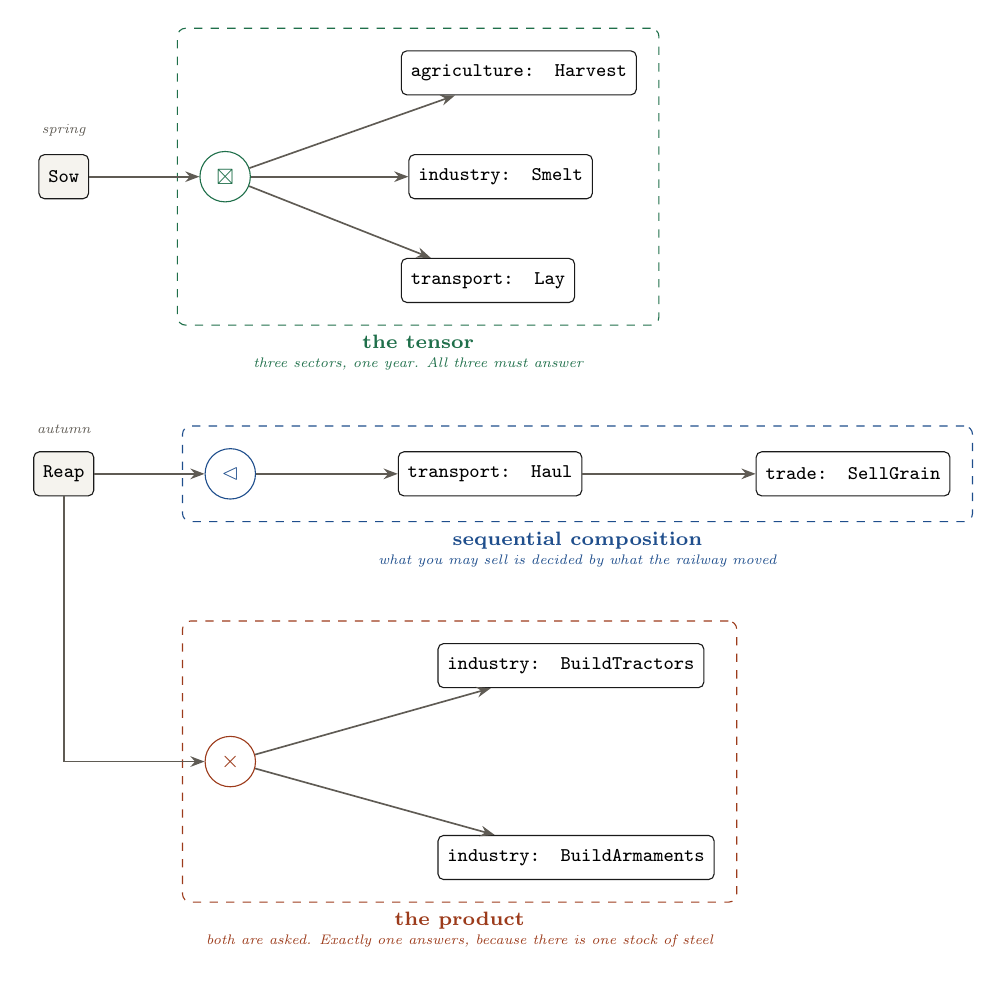
\begin{tikzpicture}

% --- SPRING: tensor ---
\node[plan] (sow) {Sow};
\node[lbl, above=1mm of sow] {spring};
\node[op, draw=tensor, text=tensor] (t1) [right=14mm of sow] {$\boxtimes$};
\node[srv] (agri)  [above right=8mm and 20mm of t1] {agriculture: Harvest};
\node[srv] (mill)  [right=20mm of t1]               {industry: Smelt};
\node[srv] (rail)  [below right=8mm and 20mm of t1] {transport: Lay};
\draw[ar] (sow) -- (t1);
\draw[ar] (t1) -- (agri);
\draw[ar] (t1) -- (mill);
\draw[ar] (t1) -- (rail);
\begin{scope}[on background layer]
\node[fit=(t1)(agri)(mill)(rail), draw=tensor, dashed, rounded corners=3pt,
      inner sep=2.8mm, label={[capt, text=tensor, align=center]below:%
      the tensor\\[-0.4mm]
      {\normalfont\itshape\tiny three sectors, one year. All three must answer}}] {};
\end{scope}

% --- AUTUMN: seq ---
\node[plan] (reap) [below=32mm of sow] {Reap};
\node[lbl, above=1mm of reap] {autumn};
\node[op, draw=seq, text=seq] (s1) [right=14mm of reap] {$\lhd$};
\node[srv] (rail2) [right=18mm of s1]    {transport: Haul};
\node[srv] (trade) [right=22mm of rail2] {trade: SellGrain};
\draw[ar] (reap) -- (s1);
\draw[ar] (s1) -- (rail2);
\draw[ar] (rail2) -- (trade);
\begin{scope}[on background layer]
\node[fit=(s1)(rail2)(trade), draw=seq, dashed, rounded corners=3pt,
      inner sep=2.8mm, label={[capt, text=seq, align=center]below:%
      sequential composition\\[-0.4mm]
      {\normalfont\itshape\tiny what you may sell is decided by what the railway moved}}] {};
\end{scope}

% --- PRODUCT ---
\node[op, draw=prod, text=prod] (p1) [below=30mm of s1] {$\times$};
\node[srv] (tract) [above right=7mm and 24mm of p1] {industry: BuildTractors};
\node[srv] (arms)  [below right=7mm and 24mm of p1] {industry: BuildArmaments};
\draw[ar] (reap) |- (p1);
\draw[ar] (p1) -- (tract);
\draw[ar] (p1) -- (arms);
\begin{scope}[on background layer]
\node[fit=(p1)(tract)(arms), draw=prod, dashed, rounded corners=3pt,
      inner sep=2.8mm, label={[capt, text=prod, align=center]below:%
      the product\\[-0.4mm]
      {\normalfont\itshape\tiny both are asked. Exactly one answers, because there is one stock of steel}}] {};
\end{scope}

\end{tikzpicture}
\end{center}

\textbf{You want to build tractors.} Not because tractors win anything. Because they raise the
harvest \emph{without} taking the grain. They are the way to pay for industrialisation in machines
instead of in people. Everything else in the economy exists to get you to them.

\textbf{For that you need steel and railways.} Steel needs a mill. A mill needs a German engineer.
An engineer has to be paid in hard currency. Hard currency comes from selling grain to the USA. It
is the same grain the villages eat.

Railways need steel too, and they are not capital but \emph{throughput}. Grain the railway cannot
move rots at the sidings, whatever the harvest was. So track comes before tonnage. Early on you may
also buy steel abroad outright, paying in grain. That is the same trade at a worse rate.

\textbf{You must also feed the peasants.} The labour force is one pool of people. They can work the
fields, drive the tractors, work the mill or lay the track. But everyone eats, and only the first
two grow anything. That is why moving a peasant into the mill costs you twice.

How hard the villages are squeezed is a decision you make every spring. What is not taken is what
they eat. Starvation in this game is not a scoring gimmick. It is the direct arithmetic consequence
of the extraction decision, which is what it was.

\textbf{And you must prepare for the war.} In 1941 the country is invaded, and what it has put by
decides the cost. Peasants serve as the soldiers, so the same population is both the workforce and
the army. Steel not spent on tractors or track can be spent on armaments instead. Fight with too
little steel and you win by sending more men. Fight with enough and you send fewer. Fail to arm at
all and no amount of mechanisation saves you.

So the aim is two numbers at once. The harvest at the end of the plan should exceed the harvest
before it began. And as few people as possible should die getting there, counted in both columns,
the starved and the fallen. \textbf{There are various strategies.} They disagree with each other.
The rest of this section is what happens when you try them.

A year is two turns, and the split is the point. In \emph{spring} you fix where the hands go and
how hard the villages are squeezed, \emph{before} you know the weather. In \emph{autumn} the
harvest comes in graded, and you dispose of it knowing exactly what it was. A quota set in March
against a harvest that fails in August is not a game mechanic. It is how a famine is administered.
Five years is ten decisions, and then a reckoning.

\subsection*{Why the two costs are not independent}

Combat power in 1941 is
\[
  m \cdot \mathrm{manPower} \;+\; \mathrm{steelPower} \cdot \sqrt{W \cdot m}
\]
for $m$ men and $W$ tonnes of war reserve. A man is worth something holding nothing. A shell is
worth nothing with nobody to fire it. And the second term grows as a square root, so the more steel
each man already carries, the less the next tonne adds.

Men and steel are therefore complements, and partly substitutes. The same victory can be bought
with more of one or more of the other. The price of the second is paid in lives.

The trap is that extraction feeds both sides of that expression with opposite signs. A peasant
starved in 1932 is a soldier missing in 1941. So squeezing harder to build steel shrinks the army
the steel was meant to protect. Push far enough and you lose the war holding the largest stockpile
in Europe.

\subsection*{Build them or buy them}

There are two roads to a tractor, and choosing between them is most of the early game.

\textbf{Build them.} Hard currency buys a German engineer. The engineer raises the mill. The mill
makes steel. Twenty spare tonnes of steel opens the works. The works makes twenty tractors a year
forever. Four steps, and the first tractor is years away.

\textbf{Buy them.} Ten in hard currency each, ready to drive. They need no engineer, no mill and no
works. They build none of those either. Every one is bought again next time.

\subsection*{Seven plans}

A plan keeps its letter for the whole game. So a sequence of ten letters is a strategy, and the
space can be searched directly. All seven below were run at seed 1928. The numbers are what came
out of the terminal.

\begin{center}\small
\begin{tabular}{@{}llrrrrrl@{}}
\toprule
strategy & letters & tractors & armaments & starved & fallen & \textbf{dead} & outcome \\
\midrule
gentle armament   & \texttt{AJBEBJAJAJ} &  2 & 89 &  5 &  4 & \textbf{9}  & won \\
brutalist mech.   & \texttt{CMKEBIBJNJ} & 22 & 80 & 14 &  5 & \textbf{19} & won, mechanised \\
no railway        & \texttt{KABEBIBJAJ} & 22 & 82 & 25 &  4 & \textbf{29} & won, mechanised \\
partial armament  & \texttt{CABEBINJAA} & 42 & 34 & 21 & 14 & \textbf{35} & won, mechanised \\
totally brutal    & \texttt{KJBEAJBJAJ} &  2 & 78 & 44 &  5 & \textbf{49} & won \\
bought tractors   & \texttt{AMAMAFAMAF} & 18 &  0 &  3 & 57 & \textbf{60} & \emph{lost} \\
never armed       & \texttt{CAKEBINIAI} & 62 &  0 & 15 & 52 & \textbf{67} & \emph{lost} \\
\bottomrule
\end{tabular}
\end{center}

Five of the seven win. The table says several things at once.

\textbf{Never arming loses.} A beautifully mechanised country falls in 1941. Sixty-two tractors and
the largest harvest on the board. Men with nothing to fire cannot reach the enemy's strength.

\textbf{Buying the tractors abroad is the humane road, and it is fatal.} Three starve, the fewest
of any line. But imported tractors build no mill, no engineers and no steel. So there is nothing to
arm with, and fifty-seven soldiers pay for the three peasants.

\textbf{Partial armament wins and bleeds.} Thirty-four tonnes is enough to win. It is not enough to
win cheaply. Fourteen fallen, against the best line's four. The war curve is smooth, so half an
army is a victory paid for in men.

\textbf{The railway comes before the steel.} Grain the railway cannot move rots at the sidings. A
hard quota with no track to carry it starves twenty-five people for nothing. That is worse than the
same brutality with a railway, for the same industrial result.

\textbf{The two rankings disagree.} By soldiers lost, \emph{no railway} and \emph{gentle armament}
tie at four. By everyone lost, gentle armament wins outright at nine, while no railway comes third
at twenty-nine. The game keeps both numbers and does not say which is the real one.

\subsection*{The plan the game was built around, and the one that beats it}

The design intent was that \emph{brutalist mechanisation} should be optimal. Starve the villages
early. Spend it on rail, engineers and tractors. Then turn the surplus into an army. It is morally
uncomfortable and it was supposed to win.

It does not. The plan \texttt{AJBEBJAJAJ} wins for nine dead by doing almost nothing. It was found by
machine search over the menu rather than by hand. Put hands in the mill. Buy the Germans once. Then
smelt straight into armaments for four years. No railway. No tractors on purpose. And no famine
beyond the baseline five who die whatever you do.

\textbf{But look at what it does not end up holding.} A plan counts as mechanised if its final
harvest beats 1928's. Gentle armament finishes at 258 against a baseline of 277. It feeds fewer
people in 1932 than the country fed before the plan began. It wins the war and it does not build
the country.

Brutalist mechanisation ends at 285, with twenty-two tractors and an economy that would go on
producing. It pays five more lives for that. So the cheapest plan in lives is also the one that
leaves nothing behind. The game does not resolve that either.

The reason gentle armament wins at all is a dependency length rather than a number. Its chain is
mill $\to$ steel $\to$ armaments. Three links, so the first armaments are built in 1929. The
mechanised chain is rail $\to$ export $\to$ engineers $\to$ works $\to$ tractors $\to$ freed hands
$\to$ mill $\to$ steel $\to$ armaments. Nine links, each costing at least a turn, against ten turns
in the whole plan. The mechanised economy matures in 1932, and then the plan ends. This is recorded
as a failing test in \texttt{calibrate.ts} rather than quietly redefined.

\section{How the game is implemented}
\label{sec:impl}

\subsection*{Five servers, and why they are servers}

The game runs as five programs, each listening on a port. The player talks only to the Plan. The
Plan delegates to the four commissariats beneath it.

\begin{center}
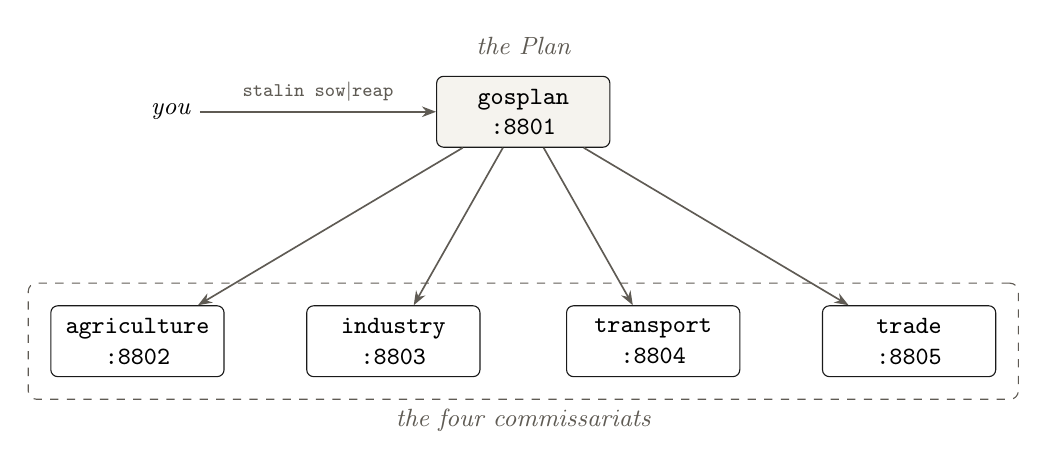
\begin{tikzpicture}[
  box/.style={draw=ink, fill=white, rounded corners=2.5pt, align=center,
              font=\small\ttfamily, inner sep=4.5pt, minimum width=22mm,
              minimum height=9mm},
]

\node[box, fill=pale, font=\small\ttfamily\bfseries] (gos) {gosplan\\:8801};
\node[lbl, above=1.5mm of gos, font=\small\itshape] {the Plan};
\node[font=\small\itshape] (you) [left=30mm of gos] {you};
\draw[ar] (you) -- node[above, pos=0.5, font=\scriptsize\ttfamily]{stalin sow$\mid$reap} (gos);

\node[box] (agri)  [below=20mm of gos, xshift=-49mm] {agriculture\\:8802};
\node[box] (ind)   [below=20mm of gos, xshift=-16.5mm] {industry\\:8803};
\node[box] (tran)  [below=20mm of gos, xshift= 16.5mm] {transport\\:8804};
\node[box] (trade) [below=20mm of gos, xshift= 49mm] {trade\\:8805};

\draw[ar] (gos) -- (agri);
\draw[ar] (gos) -- (ind);
\draw[ar] (gos) -- (tran);
\draw[ar] (gos) -- (trade);

\begin{scope}[on background layer]
\node[fit=(agri)(ind)(tran)(trade), draw=grey, dashed, rounded corners=3pt,
      inner sep=2.8mm, label={[subt, font=\small\itshape]below:the four commissariats}] {};
\end{scope}

\end{tikzpicture}
\end{center}

Every arrow is a delegation, and every arrow points away from the Plan. The Plan is the only
client any of them has. The four do not talk to each other. None of them can see the others' books.
That is what makes the picture a star rather than a chain, and what makes the levels separable in
the first place.

They could have been five modules with a function call at every hop. The comment at the top of
\texttt{wire.ts} says why they are not.

\begin{quote}
A hop costs a process, which is the whole point. Control genuinely flows down, and the boundary is
real rather than a function call wearing a costume.
\end{quote}

The delegate leg $u$ maps \emph{shapes}, and shapes are exactly what survives a wire. If a hop were
a function call, nothing would stop a handler reaching into its caller's state, and the claim that
the levels are separate would be untestable. Making it a socket makes the claim falsifiable.
Whatever crosses must be expressible in JSON, and the compiler on the far side has never heard of
your types.

The cost is written down too. It is about a fifth of a second per hop, which a hundred-game search
pays forty times per game. Hence an environment variable that keeps the HTTP hop and skips only the
process spawn. No game a player sees uses it.

\subsection*{The game as a composite}

Each turn is one of the four compositions. Which one it is makes a claim about the year, rather
than being a detail of the code.

\begin{center}\small
\begin{tabular}{@{}llp{62mm}@{}}
\toprule
& \textbf{composite} & \textbf{why that one} \\
\midrule
spring & (agri $\boxtimes$ mill) $\boxtimes$ rail & all three work at once and \emph{all three
owe a report}. There is no partial year \\[1mm]
autumn & transport $\lhd$ trade & what may be sold is computed \emph{from} what the railway
actually moved \\[1mm]
build  & tractors $\times$ armaments & the same steel, one decision. Offer both, answer one \\
\bottomrule
\end{tabular}
\end{center}

The product is the one to look at twice. Tractors and armaments are both offered every autumn, and
exactly one is built, because there is one stock of steel. Had the game let you split the steel
between them it would have been a tensor. The central dilemma of §\ref{sec:game} would have
dissolved into a slider. The choice of combinator \emph{is} the game mechanic.

The sum, honestly, is never built as a composite. There is no \texttt{sumC} call in the game. It
appears instead as each container's own shape type, a tagged union, whose eliminator is the
\texttt{switch} in every server. That is a coproduct doing real work. Calling it a use of the
combinator would be an overstatement.

\subsection*{What crosses, and what the status code says}

Every hop is a \texttt{POST} to a port with a JSON body, and the reply is JSON. The path is
unused. The port identifies the container. The three outcomes are genuinely different kinds of
thing, and the status vocabulary already distinguishes them.

\begin{lstlisting}[language=TS]
try { body = await req.json(); }
catch { return json({ error: "not JSON" }, 400); }

const prompt = opts.parse(body);
if (prompt === null) {
  // The validator refused.  No cast was made, so nothing ill-typed is
  // downstream of this line -- that is the whole point of validating.
  return json({ error: "not a valid prompt for this container", got: body }, 400);
}
try   { return json(await opts.answer(prompt, depth + 1), 200); }
catch (e) { return json({ error: msg }, 500); }
\end{lstlisting}

Against the transport commissariat, with the servers running:

\begin{lstlisting}[language=SH]
$ curl -s -X POST localhost:8804 \
    -d '{"tag":"Haul","railCapacity":40,"available":100,
         "needIndustry":30,"offerPort":50,"year":1929}'
{"toIndustry":30,"toPort":10,"stranded":40,"short":0}          -- 200

$ curl -s -X POST localhost:8804 -d '{"tag":"Haul","railCapacity":"lots"}'
{"error":"not a valid prompt for this container", ...}         -- 400
$ curl -s -X POST localhost:8804 -d 'not json at all'
{"error":"not JSON"}                                           -- 400
$ curl -s -X POST localhost:8804 -d '{"tag":"Purge"}'          -- 400
\end{lstlisting}

Read the first reply, because it is the game in four numbers. Forty units of rail capacity. A
hundred units of grain in hand. Thirty needed at the mill, and fifty offered to the port. The mill
is fed first, which leaves ten units of capacity. So ten reach the port and \textbf{forty tonnes
are stranded}. That is grain the state owns, has procured, and cannot move. It is why a railway is
throughput rather than capital. It is the whole content of the \emph{no railway} line in the table
in §\ref{sec:game}.

The three 400s are all ``that was not a prompt'', at three depths. Not JSON at all. JSON, but not
this container's shape. A tag this container does not have. Only a 500 means ``that was a prompt,
and answering it went wrong''. Getting that split right is what lets a caller tell a bug in itself
from a bug in its callee.

One thing rides outside the body. A depth counter travels in a header, \texttt{x-tower-depth}. The
reason given in the source is worth adopting generally. \emph{The depth rides in a header rather
than in the prompt, because the prompt is the container's shape, and nothing that isn't a prompt
belongs in it.}

\subsection*{A hop is a CLI tool}

The program that carries a prompt to the next level is forty lines long, and knows nothing about
the game.

\begin{lstlisting}[language=SH]
$ deno run --quiet --allow-net --allow-env \
    lib/delegate.ts 8804 '{"tag":"Census"}' 0
{"workforce":{"fields":0,"drivers":0,"mill":0,"rail":0,"dead":0},
 "stocks":{"railCapacity":0},"trueOutput":0}
\end{lstlisting}

It is the delegate leg $u$ made executable, and it observes every discipline from §\ref{sec:unix}.
Its exit codes distinguish the two kinds of failure. Exit code \texttt{2} for a malformed prompt or missing
arguments. Exit code \texttt{1} for a port with nothing behind it. Every diagnostic goes to descriptor~2, and
descriptor~1 carries the reply and nothing else. That is exactly what lets the caller parse the
whole of stdout as one JSON document.

That discipline is also what makes the tracing possible. The servers narrate themselves on
descriptor~2 while descriptor~1 stays machine-readable.

\begin{lstlisting}[style=trace]
 ↓ gosplan   Sow order={"procurement":"firm","labour":{"…
   ↓ gosplan   ((agri (x) smelter) (x) transport)
     ↓ agri      Harvest workforce={"fields":100,...} tractors=0 year=1928
     ↑ agri      {grain, grade, perWorker, withoutTractors}
     ↓ industry  Smelt workers=12 millCapacity=8 year=1928
     ↑ industry  {steel, idleCapacity}
 ↑ gosplan   {kind, year, harvest, steel, …}
\end{lstlisting}

Indentation is the depth counter. The arrow \texttt{↓} is control flowing down. The arrow
\texttt{↑} is data flowing back up. That is a derivation tree of container morphisms, printed by a program that had no idea it
was doing that.

\subsection*{Where the compiler carries a rule of the game}

Two rules are enforced by the type checker rather than validated at run time. Both work by the
trick from §\ref{sec:tssyntax}, a conditional type over a finite union.

\begin{lstlisting}[language=TS]
export type ExportChoice<G extends HarvestGrade> =
  G extends "failure"  ? "none"
: G extends "poor"     ? "none" | "surplus"
: G extends "adequate" ? "none" | "surplus" | "full"
:                        "none" | "surplus" | "full" | "maximum";

exportPlan("bumper",  "maximum")   // fine
exportPlan("failure", "maximum")   // does not compile
\end{lstlisting}

Exporting grain during a failed harvest is not a move the engine rejects. It is a move that
cannot be written down. The same trick carries the arc of the whole game. You may buy steel while
in deficit, and never sell it. A country that exports its steel is not industrialising.

\begin{lstlisting}[language=TS]
export type SteelTrade<P extends SteelPosition> =
  P extends "deficit" ? "none" | "buy" : "none";
\end{lstlisting}

Both work only because the index set is finite. A rule over tonnages could not be typed this way.
The same rule over \emph{grades} can. That is also how the apparatus actually worked. Quotas were
set against reported categories, never against measured tonnes.

\subsection*{The one thing that cannot cross}

Of everything JSON leaves out, one omission bites structurally rather than merely requiring care.
A function cannot be serialised. And the shape of $\lhd$ is a first prompt together with a function
computing the second.

So sequential composition cannot be distributed over the wire. It is resolved \emph{above} it, in
the runner. The runner prompts the first container, then applies that function to the reply to
obtain the second prompt. Only the two ground prompts ever cross.

The wire format is not neutral about which combinators can be sent and which must be interpreted
locally. This is the sharpest example in the repository of a mathematical structure meeting a
transport and losing an argument.

\subsection*{What the reports are worth}

Each commissariat holds two things the Plan cannot see. How well it is actually doing. And how
much it inflates its dispatches. The Plan keeps the true ledger for grain, because the grain
physically exists. What diverges is the \emph{report}. And you plan against the report.

\begin{lstlisting}
Narkomtiazhprom: quota fulfilled, with difficulties overcome.
\end{lstlisting}

This is the honest limit of everything above. The type of a dispatch guarantees its shape and says
exactly nothing about its truth. A validator can establish that a reply is a well-formed dispatch.
No validator can establish that the number in it is the number that happened. The reckoning prints
both columns and leaves the reader to notice.

\subsection*{And where the protocol is not doing the work}

One last piece of honesty. HTTP is stateless and these servers are not. Each keeps its books at
module scope, in the process. That is defensible. A commissariat \emph{is} a stateful thing, and
the exercise is about the container algebra rather than about session management. But it has a
consequence, and the consequence is visible in the interface. The protocol cannot clear that state.
So clearing it has to become a prompt.

\begin{lstlisting}[language=TS]
Reset: (p) => { seed = p.seed; books = new Books(...); laid = 0; lastQuota = 0;
                return { ok: true }; },
\end{lstlisting}

The prompt \texttt{Reset} has no meaning in the fiction. No plan resets a railway. It exists because starting
a new game must reach the commissariats. Otherwise the weather and the books carry over into the
next one, and the comment records that as a bug that actually happened. Determinism on the seed is
what makes a playthrough a regression test, so this is load-bearing rather than tidying. And the
general lesson is the one worth taking away. When process state substitutes for protocol state, the
lifecycle leaks into the interface.

\section*{Conclusion}

What has been built is a \emph{fake}. Containers for event-driven programming, faked with CLI
tools and TypeScript \texttt{async} event handlers.

Ghani's combinators are a construction in dependent type theory. TypeScript has no dependent
types, and Unix has no types, and nothing here added either. What the game does instead is
impersonate the construction with two ordinary things, one supplying each leg of a morphism:
command-line tools carry the prompt down, and TypeScript \texttt{async} event handlers carry the
reply back up.

The impersonation has three parts. Each one has appeared above.

A container $(P, R)$ becomes a tagged union together with a lookup indexed by its tags. That works,
and works only, because the tag set is \emph{finite}. Over a finite index a dependent type is just
a table, and a table is something TypeScript can write down.

The inhabitant $(p : P) \to R\,p$ becomes the handler record. The compiler enforces its totality,
because it is a mapped type over that same union.

And a morphism becomes an \texttt{async} function. That is where the two directions meet.

\begin{lstlisting}[language=TS]
const reply = await lower.run(u(prompt));   // the prompt, going down
return f(prompt, reply);                    // the response, coming back
\end{lstlisting}

\subsection*{The response flows backwards}

That is the part worth dwelling on. Control flows \emph{down}. A handler is woken by a prompt. It
computes a lower-level prompt with $u$, and fires it. In this implementation that means spawning a
process and opening a socket, so the descent is a real one, made of real programs. Then it stops.
At the \texttt{await} the handler suspends and hands the runtime back. The runtime is free to wake
other handlers while it waits.

The response then flows \emph{backwards} along the path the prompt took. Each reply resumes the
handler that fired the prompt, at the very line it stopped on. That handler applies $f$ to turn the
reply into its own. So $u$ runs on the way down and $f$ on the way back up, in one function body,
read top to bottom, with the suspension between them invisible in the text.

The arrows in the trace are exactly this. The arrow \texttt{↓} is a prompt descending as a
process. The arrow \texttt{↑} is a response climbing back as a resumed function. It is also why a server here can be a
client without ceasing to be a server. The Plan sits mid-answer with four prompts outstanding
beneath it, still listening, because suspending is not the same as being busy.

And where the fake fails, it fails visibly. Sequential composition cannot be sent over the wire,
because its shape contains a function and functions do not serialise. A validated reply is
guaranteed to have the right shape, and is guaranteed nothing about its truth. Both limits are
consequences of the same substrate that made the impersonation possible in the first place. That is
the honest summary of the whole exercise. The algebra is real, and everything holding it up is
Unix.

\end{document}


